% Options for packages loaded elsewhere
\PassOptionsToPackage{unicode}{hyperref}
\PassOptionsToPackage{hyphens}{url}
%
\documentclass[
  12pt,
  a4paper,
  DIV=11,
  numbers=noendperiod]{scrreprt}

\usepackage{amsmath,amssymb}
\usepackage{setspace}
\usepackage{iftex}
\ifPDFTeX
  \usepackage[T1]{fontenc}
  \usepackage[utf8]{inputenc}
  \usepackage{textcomp} % provide euro and other symbols
\else % if luatex or xetex
  \usepackage{unicode-math}
  \defaultfontfeatures{Scale=MatchLowercase}
  \defaultfontfeatures[\rmfamily]{Ligatures=TeX,Scale=1}
\fi
\usepackage{lmodern}
\ifPDFTeX\else  
    % xetex/luatex font selection
\fi
% Use upquote if available, for straight quotes in verbatim environments
\IfFileExists{upquote.sty}{\usepackage{upquote}}{}
\IfFileExists{microtype.sty}{% use microtype if available
  \usepackage[]{microtype}
  \UseMicrotypeSet[protrusion]{basicmath} % disable protrusion for tt fonts
}{}
\usepackage{xcolor}
\setlength{\emergencystretch}{3em} % prevent overfull lines
\setcounter{secnumdepth}{5}
% Make \paragraph and \subparagraph free-standing
\ifx\paragraph\undefined\else
  \let\oldparagraph\paragraph
  \renewcommand{\paragraph}[1]{\oldparagraph{#1}\mbox{}}
\fi
\ifx\subparagraph\undefined\else
  \let\oldsubparagraph\subparagraph
  \renewcommand{\subparagraph}[1]{\oldsubparagraph{#1}\mbox{}}
\fi

\usepackage{color}
\usepackage{fancyvrb}
\newcommand{\VerbBar}{|}
\newcommand{\VERB}{\Verb[commandchars=\\\{\}]}
\DefineVerbatimEnvironment{Highlighting}{Verbatim}{commandchars=\\\{\}}
% Add ',fontsize=\small' for more characters per line
\usepackage{framed}
\definecolor{shadecolor}{RGB}{241,243,245}
\newenvironment{Shaded}{\begin{snugshade}}{\end{snugshade}}
\newcommand{\AlertTok}[1]{\textcolor[rgb]{0.68,0.00,0.00}{#1}}
\newcommand{\AnnotationTok}[1]{\textcolor[rgb]{0.37,0.37,0.37}{#1}}
\newcommand{\AttributeTok}[1]{\textcolor[rgb]{0.40,0.45,0.13}{#1}}
\newcommand{\BaseNTok}[1]{\textcolor[rgb]{0.68,0.00,0.00}{#1}}
\newcommand{\BuiltInTok}[1]{\textcolor[rgb]{0.00,0.23,0.31}{#1}}
\newcommand{\CharTok}[1]{\textcolor[rgb]{0.13,0.47,0.30}{#1}}
\newcommand{\CommentTok}[1]{\textcolor[rgb]{0.37,0.37,0.37}{#1}}
\newcommand{\CommentVarTok}[1]{\textcolor[rgb]{0.37,0.37,0.37}{\textit{#1}}}
\newcommand{\ConstantTok}[1]{\textcolor[rgb]{0.56,0.35,0.01}{#1}}
\newcommand{\ControlFlowTok}[1]{\textcolor[rgb]{0.00,0.23,0.31}{#1}}
\newcommand{\DataTypeTok}[1]{\textcolor[rgb]{0.68,0.00,0.00}{#1}}
\newcommand{\DecValTok}[1]{\textcolor[rgb]{0.68,0.00,0.00}{#1}}
\newcommand{\DocumentationTok}[1]{\textcolor[rgb]{0.37,0.37,0.37}{\textit{#1}}}
\newcommand{\ErrorTok}[1]{\textcolor[rgb]{0.68,0.00,0.00}{#1}}
\newcommand{\ExtensionTok}[1]{\textcolor[rgb]{0.00,0.23,0.31}{#1}}
\newcommand{\FloatTok}[1]{\textcolor[rgb]{0.68,0.00,0.00}{#1}}
\newcommand{\FunctionTok}[1]{\textcolor[rgb]{0.28,0.35,0.67}{#1}}
\newcommand{\ImportTok}[1]{\textcolor[rgb]{0.00,0.46,0.62}{#1}}
\newcommand{\InformationTok}[1]{\textcolor[rgb]{0.37,0.37,0.37}{#1}}
\newcommand{\KeywordTok}[1]{\textcolor[rgb]{0.00,0.23,0.31}{#1}}
\newcommand{\NormalTok}[1]{\textcolor[rgb]{0.00,0.23,0.31}{#1}}
\newcommand{\OperatorTok}[1]{\textcolor[rgb]{0.37,0.37,0.37}{#1}}
\newcommand{\OtherTok}[1]{\textcolor[rgb]{0.00,0.23,0.31}{#1}}
\newcommand{\PreprocessorTok}[1]{\textcolor[rgb]{0.68,0.00,0.00}{#1}}
\newcommand{\RegionMarkerTok}[1]{\textcolor[rgb]{0.00,0.23,0.31}{#1}}
\newcommand{\SpecialCharTok}[1]{\textcolor[rgb]{0.37,0.37,0.37}{#1}}
\newcommand{\SpecialStringTok}[1]{\textcolor[rgb]{0.13,0.47,0.30}{#1}}
\newcommand{\StringTok}[1]{\textcolor[rgb]{0.13,0.47,0.30}{#1}}
\newcommand{\VariableTok}[1]{\textcolor[rgb]{0.07,0.07,0.07}{#1}}
\newcommand{\VerbatimStringTok}[1]{\textcolor[rgb]{0.13,0.47,0.30}{#1}}
\newcommand{\WarningTok}[1]{\textcolor[rgb]{0.37,0.37,0.37}{\textit{#1}}}

\providecommand{\tightlist}{%
  \setlength{\itemsep}{0pt}\setlength{\parskip}{0pt}}\usepackage{longtable,booktabs,array}
\usepackage{calc} % for calculating minipage widths
% Correct order of tables after \paragraph or \subparagraph
\usepackage{etoolbox}
\makeatletter
\patchcmd\longtable{\par}{\if@noskipsec\mbox{}\fi\par}{}{}
\makeatother
% Allow footnotes in longtable head/foot
\IfFileExists{footnotehyper.sty}{\usepackage{footnotehyper}}{\usepackage{footnote}}
\makesavenoteenv{longtable}
\usepackage{graphicx}
\makeatletter
\def\maxwidth{\ifdim\Gin@nat@width>\linewidth\linewidth\else\Gin@nat@width\fi}
\def\maxheight{\ifdim\Gin@nat@height>\textheight\textheight\else\Gin@nat@height\fi}
\makeatother
% Scale images if necessary, so that they will not overflow the page
% margins by default, and it is still possible to overwrite the defaults
% using explicit options in \includegraphics[width, height, ...]{}
\setkeys{Gin}{width=\maxwidth,height=\maxheight,keepaspectratio}
% Set default figure placement to htbp
\makeatletter
\def\fps@figure{htbp}
\makeatother

% s\usepackage{juliamono}
\usepackage{indentfirst}
\usepackage{float}
\floatplacement{figure}{H}
\IfFileExists{plex-otf.sty}{
  %% Full TeXlive
  \usepackage[
    % math,
    RM={Scale=0.94},SS={Scale=0.94},SScon={Scale=0.94},TT={Scale=MatchLowercase,FakeStretch=0.9},
    DefaultFeatures={Ligatures=Common}
  ]{plex-otf}
  % \usepackage[Scale=MatchUppercase]{juliamono}
}{
  %% TinyTeX
  \usepackage{libertine}
}
\KOMAoption{captions}{tableheading}
\makeatletter
\@ifpackageloaded{caption}{}{\usepackage{caption}}
\AtBeginDocument{%
\ifdefined\contentsname
  \renewcommand*\contentsname{Содержание}
\else
  \newcommand\contentsname{Содержание}
\fi
\ifdefined\listfigurename
  \renewcommand*\listfigurename{Список иллюстраций}
\else
  \newcommand\listfigurename{Список иллюстраций}
\fi
\ifdefined\listtablename
  \renewcommand*\listtablename{Список таблиц}
\else
  \newcommand\listtablename{Список таблиц}
\fi
\ifdefined\figurename
  \renewcommand*\figurename{Рисунок}
\else
  \newcommand\figurename{Рисунок}
\fi
\ifdefined\tablename
  \renewcommand*\tablename{Таблица}
\else
  \newcommand\tablename{Таблица}
\fi
}
\@ifpackageloaded{float}{}{\usepackage{float}}
\floatstyle{ruled}
\@ifundefined{c@chapter}{\newfloat{codelisting}{h}{lop}}{\newfloat{codelisting}{h}{lop}[chapter]}
\floatname{codelisting}{Список}
\newcommand*\listoflistings{\listof{codelisting}{Листинги}}
\makeatother
\makeatletter
\makeatother
\makeatletter
\@ifpackageloaded{caption}{}{\usepackage{caption}}
\@ifpackageloaded{subcaption}{}{\usepackage{subcaption}}
\makeatother
\ifLuaTeX
\usepackage[bidi=basic]{babel}
\else
\usepackage[bidi=default]{babel}
\fi
\babelprovide[main,import]{russian}
\babelprovide[import]{english}
% get rid of language-specific shorthands (see #6817):
\let\LanguageShortHands\languageshorthands
\def\languageshorthands#1{}
\ifLuaTeX
  \usepackage{selnolig}  % disable illegal ligatures
\fi
\usepackage[style=gost-numeric,backend=biber,langhook=extras,autolang=other*]{biblatex}
\addbibresource{bib/cite.bib}
\usepackage{csquotes}
\usepackage{bookmark}

\IfFileExists{xurl.sty}{\usepackage{xurl}}{} % add URL line breaks if available
\urlstyle{same} % disable monospaced font for URLs
\hypersetup{
  pdftitle={Отчёта по лабораторной работе1},
  pdfauthor={Нджову Нелиа},
  pdflang={ru-RU},
  hidelinks,
  pdfcreator={LaTeX via pandoc}}

\title{Отчёта по лабораторной работе1}
\usepackage{etoolbox}
\makeatletter
\providecommand{\subtitle}[1]{% add subtitle to \maketitle
  \apptocmd{\@title}{\par {\large #1 \par}}{}{}
}
\makeatother
\subtitle{Математическое моделирование}
\author{Нджову Нелиа}
\date{}

\begin{document}
\maketitle

\renewcommand*\contentsname{Содержание}
{
\setcounter{tocdepth}{1}
\tableofcontents
}
\listoffigures
\listoftables
\setstretch{1.5}
\chapter{Цель
работы}\label{ux446ux435ux43bux44c-ux440ux430ux431ux43eux442ux44b}

Изучить модель экспоненциального роста, провести параметрическое
исследование влияния коэффициента роста αα на динамику системы, а также
освоить современные практики воспроизводимых исследований (литературное
программирование, DrWatson, Git) при выполнении лабораторных работ.

\chapter{Задание}\label{ux437ux430ux434ux430ux43dux438ux435}

\begin{enumerate}
\def\labelenumi{\arabic{enumi}.}
\item
  Настройка git
\item
  Рабочее пространство лабораторной работы
\item
  Создание проекта DrWatson для лабораторных
\item
  Модель экспоненциального роста
\end{enumerate}

\chapter{Выполнение лабораторной
работы}\label{ux432ux44bux43fux43eux43bux43dux435ux43dux438ux435-ux43bux430ux431ux43eux440ux430ux442ux43eux440ux43dux43eux439-ux440ux430ux431ux43eux442ux44b}

\section{1. Настройка
git}\label{ux43dux430ux441ux442ux440ux43eux439ux43aux430-git}

Из моих предыдущих лабораторных работ я уже установил git и gh и
выполнил базовую настройку. Итак, для этой лабораторной работы я начал с
создания учетной записи на gitverse и заполнения необходимой
информации(рис.1).

\begin{figure}

\centering{

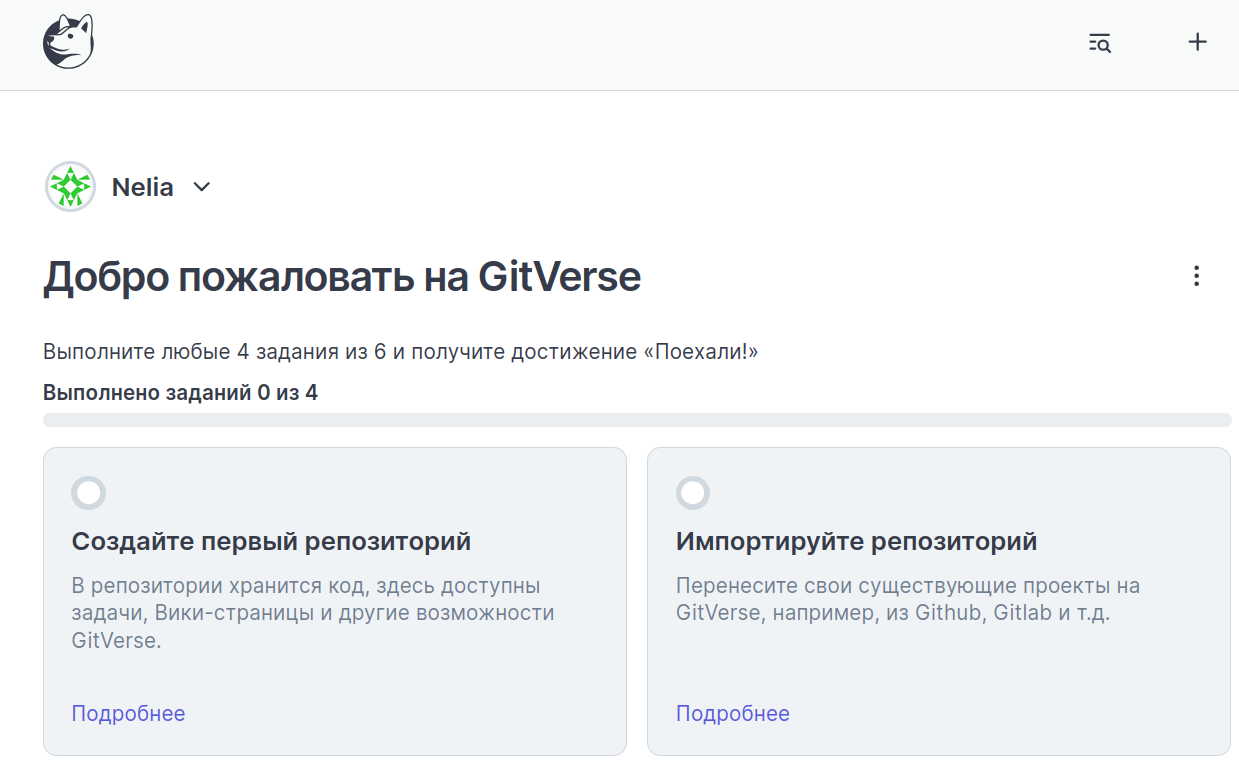
\includegraphics[width=0.7\textwidth,height=\textheight]{image/fig-002.png}

}

\caption{\label{fig-001}Создание учетной записи на gitverse}

\end{figure}%

Я авторизуюсь с помощью команды gh auth login. Утилита задала мне
несколько вопросов, и в итоге я авторизовался через браузер(рис.2)

\begin{figure}

\centering{

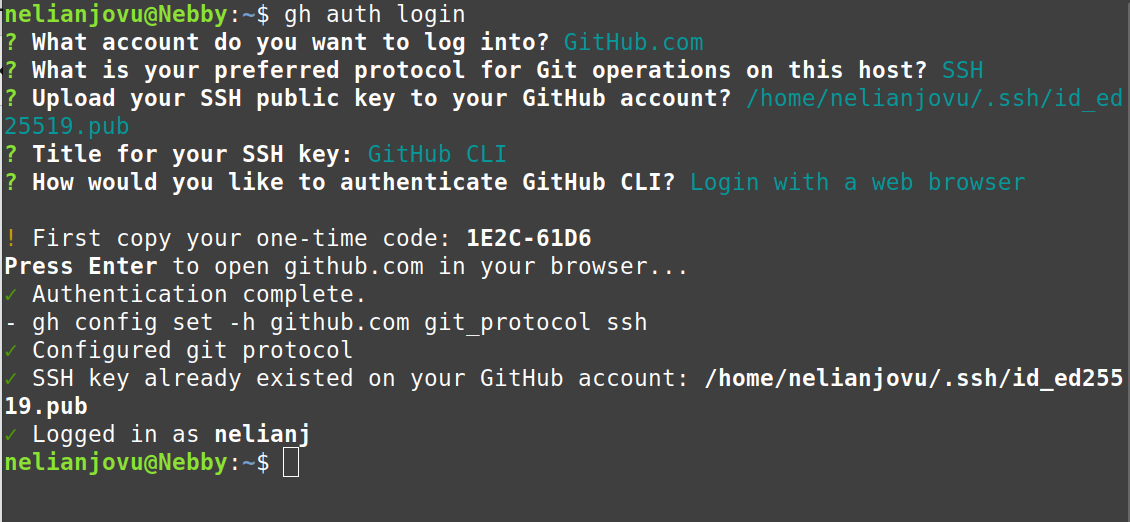
\includegraphics[width=0.7\textwidth,height=\textheight]{image/fig-005.png}

}

\caption{\label{fig-002}Авторизация учетной записи}

\end{figure}%

Я создаю ключ ssh для доступа к github(рис.3)

\begin{figure}

\centering{


\includegraphics[width=0.7\textwidth,height=\textheight]{image/fig-007.png}

}

\caption{\label{fig-003}Ключ для доступа к github}

\end{figure}%

Я добавляю ключ ssh в агента(рис. 4)

\begin{figure}

\centering{


\includegraphics[width=0.7\textwidth,height=\textheight]{image/fig-008.png}

}

\caption{\label{fig-004}Добавление ключа в агента}

\end{figure}%

Я добавляю ключ ssh к вашей учетной записи на gitverse через
веб-интерфейс. Затем используйте команду, чтобы добавить ключ ssh к
вашей учетной записи на github(рис. 5 и 6)

\begin{figure}

\centering{

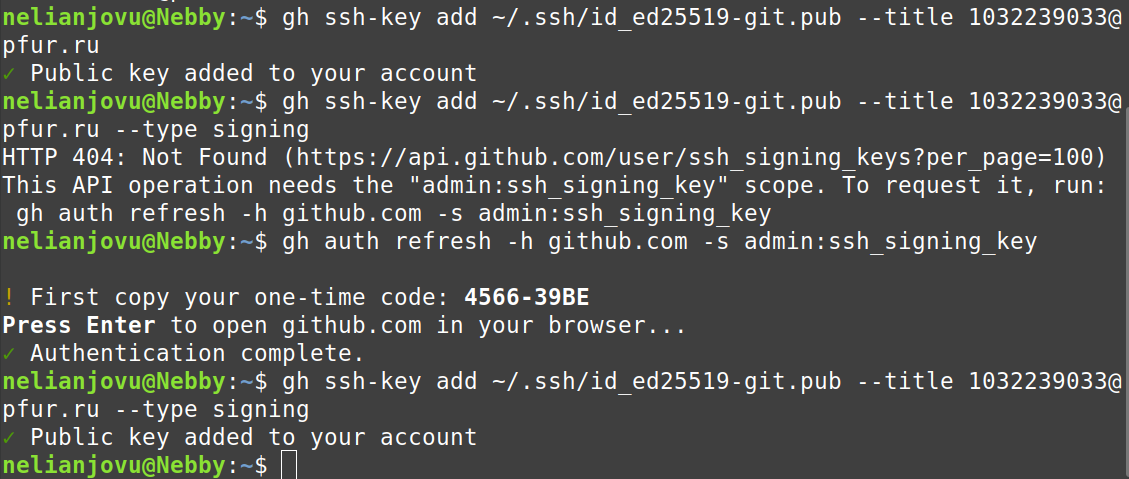
\includegraphics[width=0.7\textwidth,height=\textheight]{image/fig-011.png}

}

\caption{\label{fig-005}Добавление ключа на gitverse}

\end{figure}%

\begin{figure}

\centering{

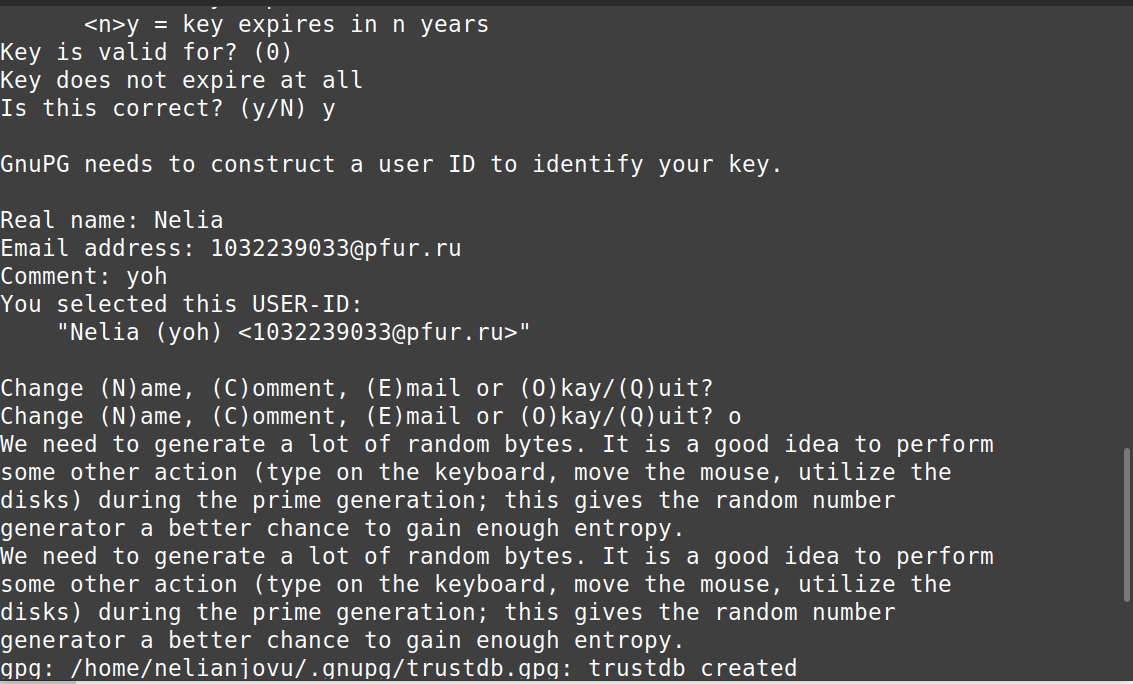
\includegraphics[width=0.7\textwidth,height=\textheight]{image/fig-013.png}

}

\caption{\label{fig-006}Добавление ключа на github}

\end{figure}%

Я генерирую ключ gpg, выбирая параметры, указанные в руководстве по
лабораторной работе(рис. 7)

\begin{figure}

\centering{

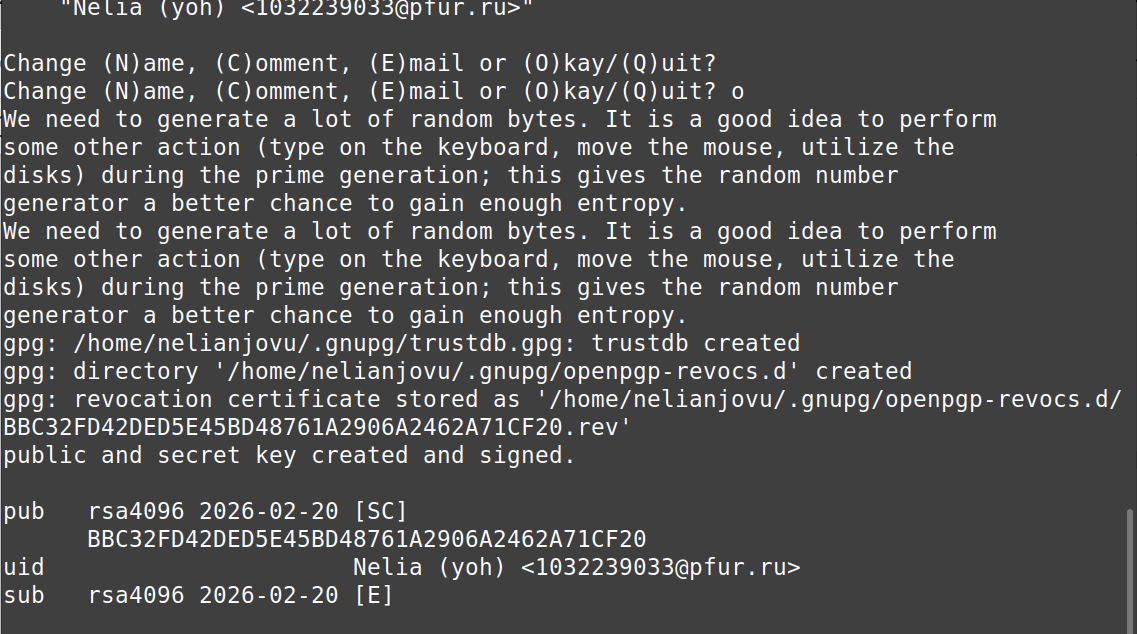
\includegraphics[width=0.7\textwidth,height=\textheight]{image/fig-014.png}

}

\caption{\label{fig-007}генерация ключа gpg}

\end{figure}%

Я вывожу список ключей и копирую отпечаток пальца (который находится под
строкой, начинающейся с sec) закрытого ключа.(рис. 8)

\begin{figure}

\centering{

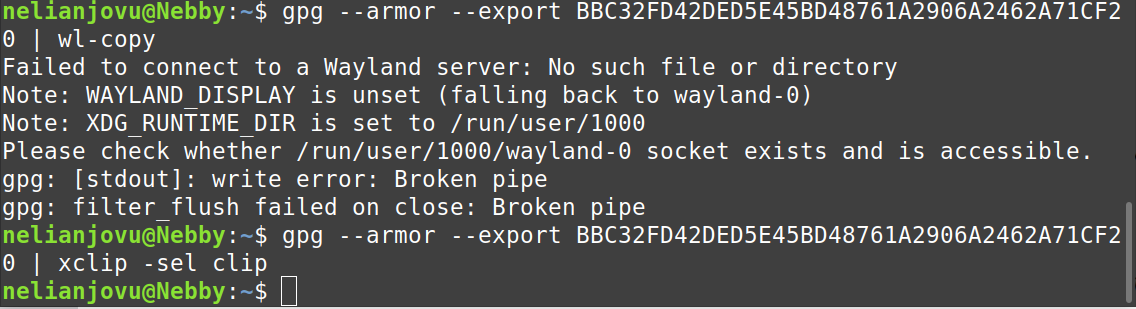
\includegraphics[width=0.7\textwidth,height=\textheight]{image/fig-017.png}

}

\caption{\label{fig-008}список ключей}

\end{figure}%

Я копирую сгенерированный PGP-ключ в буфер обмена. Я использую xclip,
потому что wl-copy выдал ошибку(рис. 9)

\begin{figure}

\centering{

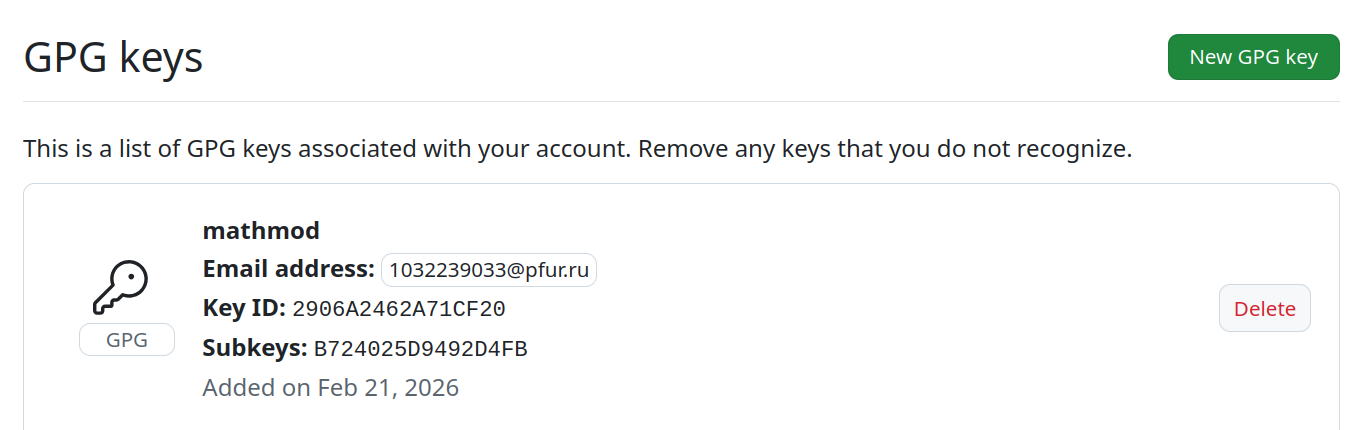
\includegraphics[width=0.7\textwidth,height=\textheight]{image/fig-019.png}

}

\caption{\label{fig-009}копирование ключа}

\end{figure}%

Я добавляю сгенерированный ключ gpg в github и gitverse(рис. 10 и 11)

\begin{figure}

\centering{

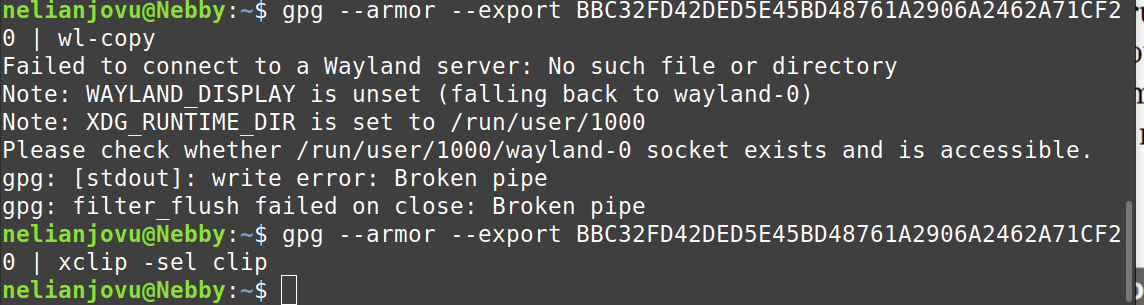
\includegraphics[width=0.7\textwidth,height=\textheight]{image/fig-020.png}

}

\caption{\label{fig-010}Добавление ключа на gitverse}

\end{figure}%

\begin{figure}

\centering{

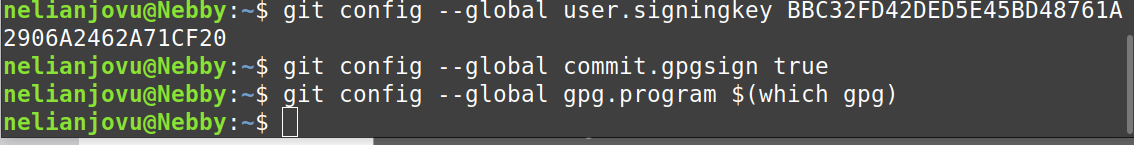
\includegraphics[width=0.7\textwidth,height=\textheight]{image/fig-021.png}

}

\caption{\label{fig-011}Добавление ключа на github}

\end{figure}%

Используя электронное письмо, подключенное к моей учетной записи, я
говорю Git использовать его при подписании коммитов(рис. 12)

\begin{figure}

\centering{

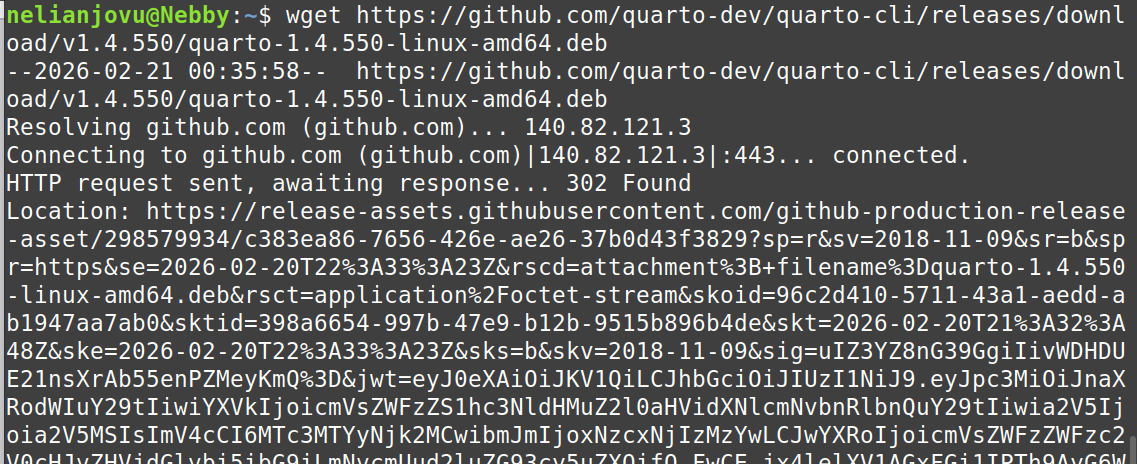
\includegraphics[width=0.7\textwidth,height=\textheight]{image/fig-023.png}

}

\caption{\label{fig-012}автоматические подписи git-коммитов}

\end{figure}%

\section{2. Рабочее пространство лабораторной
работы}\label{ux440ux430ux431ux43eux447ux435ux435-ux43fux440ux43eux441ux442ux440ux430ux43dux441ux442ux432ux43e-ux43bux430ux431ux43eux440ux430ux442ux43eux440ux43dux43eux439-ux440ux430ux431ux43eux442ux44b}

Я устанавливаю пакет, который поставляется с инструментами разработки
для linux mint(рис. 13)

\begin{figure}

\centering{

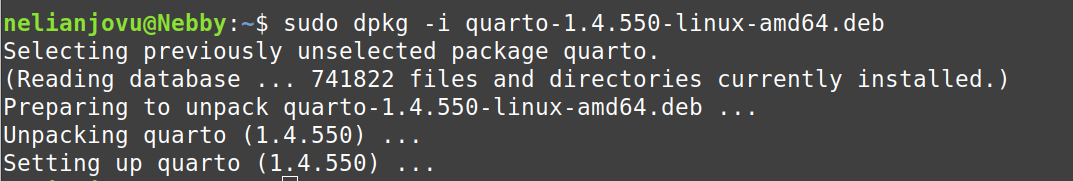
\includegraphics[width=0.7\textwidth,height=\textheight]{image/fig-024.png}

}

\caption{\label{fig-013}уствновка инструменты разработки}

\end{figure}%

Затем я устанавливаю quarto. Quarto - это инструмент для научной
публикации с открытым исходным кодом, который позволяет создавать
профессиональные отчеты, объединяя текст, код и результаты в одном
документе, с поддержкой Julia, Python и R(рис. 14)

\begin{figure}

\centering{

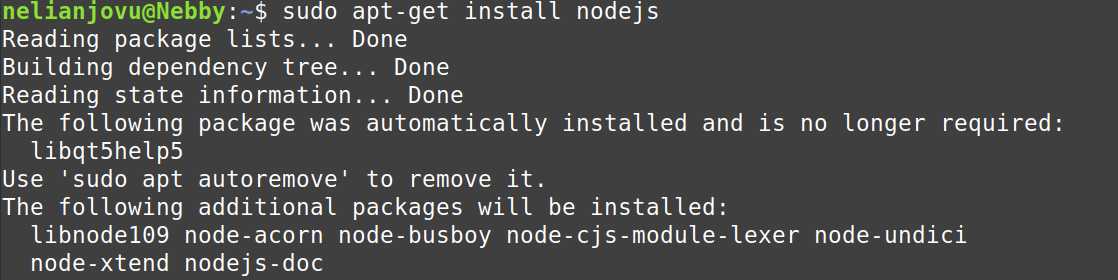
\includegraphics[width=0.7\textwidth,height=\textheight]{image/fig-025.png}

}

\caption{\label{fig-014}уствновка quarto}

\end{figure}%

Наконец, я устанавливаю nodejs, yarn и pnpm(рис. 15, 16 и 17)

\begin{figure}

\centering{

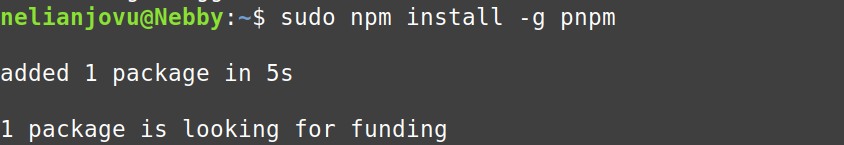
\includegraphics[width=0.7\textwidth,height=\textheight]{image/fig-027.png}

}

\caption{\label{fig-015}уствновка nodejs}

\end{figure}%

\begin{figure}

\centering{

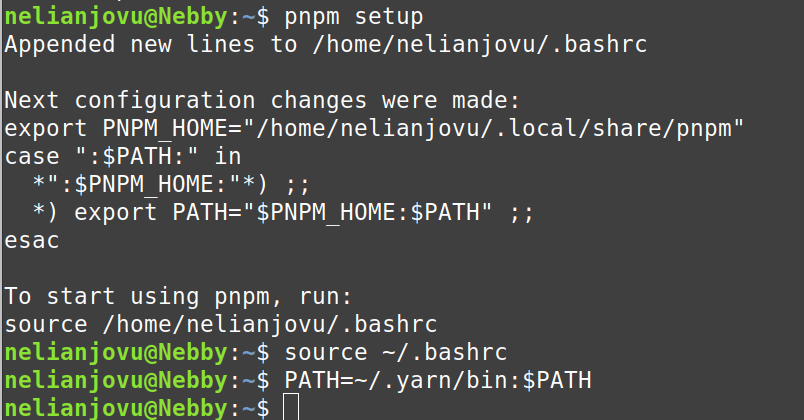
\includegraphics[width=0.7\textwidth,height=\textheight]{image/fig-028.png}

}

\caption{\label{fig-016}уствновка yarn}

\end{figure}%

\begin{figure}

\centering{

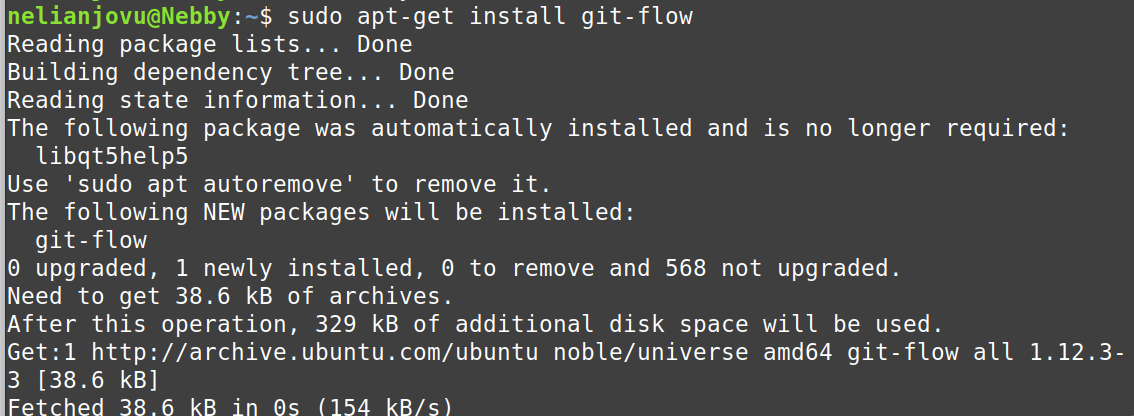
\includegraphics[width=0.7\textwidth,height=\textheight]{image/fig-029.png}

}

\caption{\label{fig-017}уствновка pnpm}

\end{figure}%

Для работы с Node.js Я добавляю каталог с исполняемыми файлами,
установленными менеджером пакетов, в переменную PATH(рис. 18)

\begin{figure}

\centering{

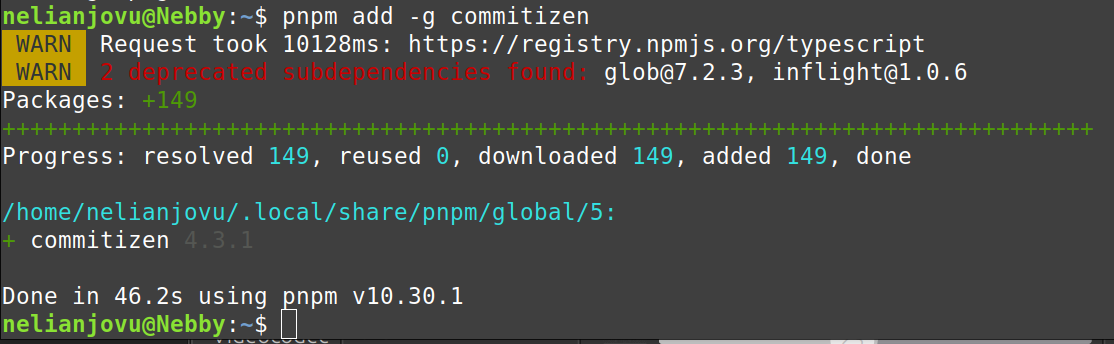
\includegraphics[width=0.7\textwidth,height=\textheight]{image/fig-030.png}

}

\caption{\label{fig-018}настройка nodejs}

\end{figure}%

Я устанавливаю gitflow. Gitflow - это модель ветвления для Git, которая
обеспечивает структурированный рабочий процесс с использованием
выделенных ветвей для функций, релизов и исправлений, помогая командам
управлять параллельной разработкой и поддерживать стабильный код(рис.
19)

\begin{figure}

\centering{

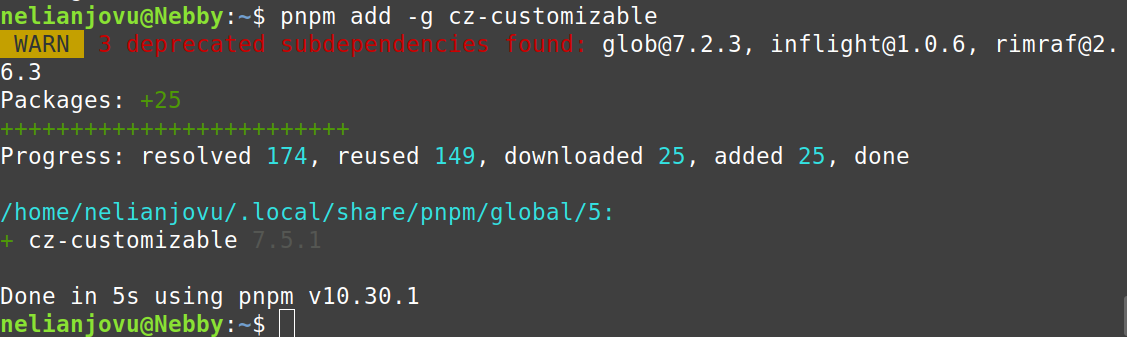
\includegraphics[width=0.7\textwidth,height=\textheight]{image/fig-031.png}

}

\caption{\label{fig-019}уствновка gitflow}

\end{figure}%

Следуя инструкциям руководства, я использую команды, которые помогают
форматировать коммиты, одновременно с этим устанавливается git-cz,
который мы будем использовать для коммитов(рис. 20)

\begin{figure}

\centering{

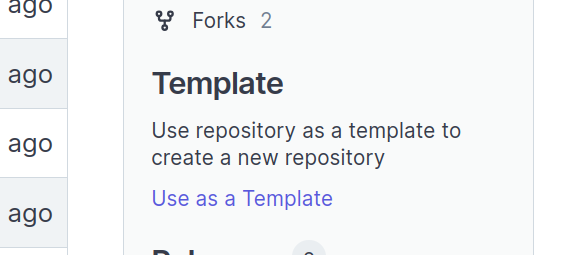
\includegraphics[width=0.7\textwidth,height=\textheight]{image/fig-033.png}

}

\caption{\label{fig-020}форматировка коммиты}

\end{figure}%

Команда на скриншоте позволяет мне более глубоко настроить
форматирование коммитов(рис. 21)

\begin{figure}

\centering{

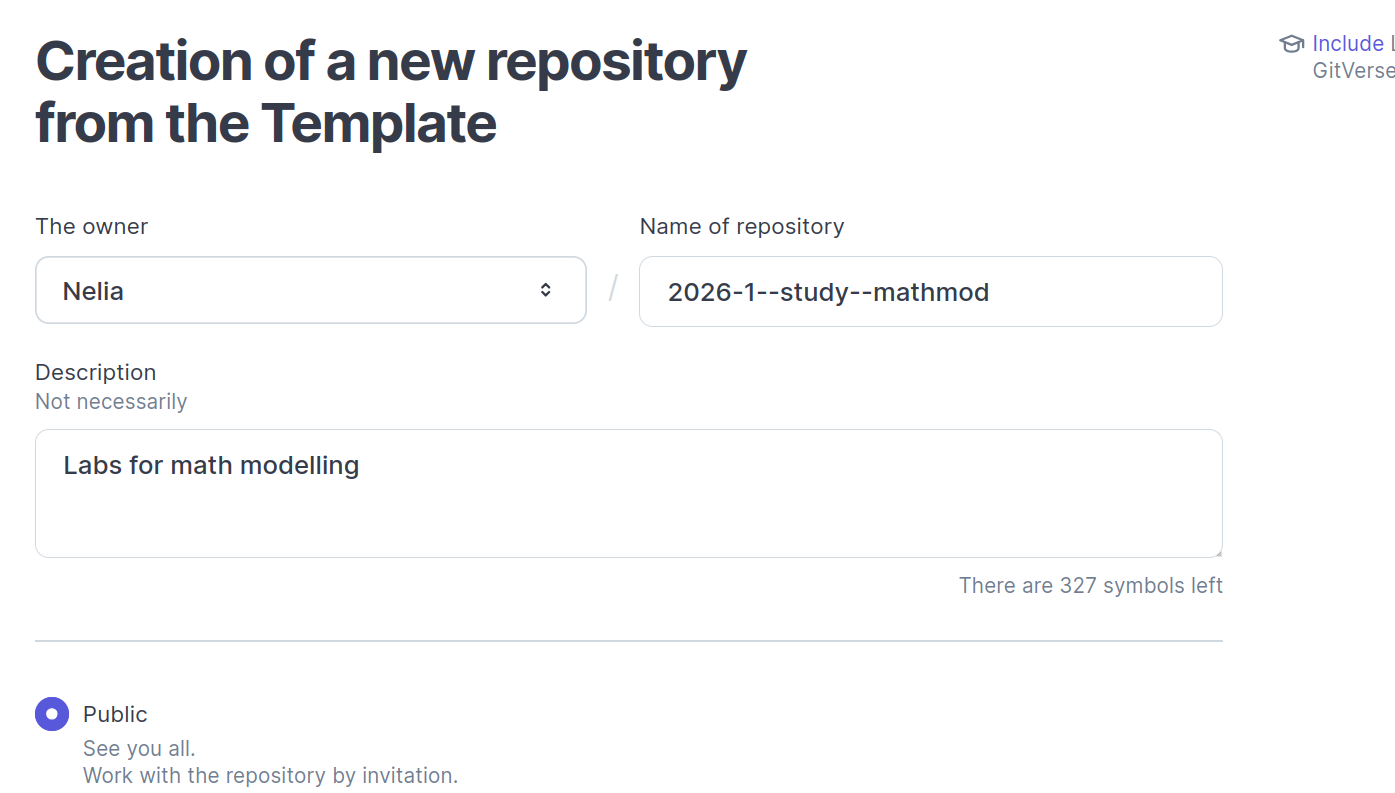
\includegraphics[width=0.7\textwidth,height=\textheight]{image/fig-034.png}

}

\caption{\label{fig-021}форматировка коммиты}

\end{figure}%

Эта команда автоматизирует изменение номера версии(рис. 22)

\begin{figure}

\centering{

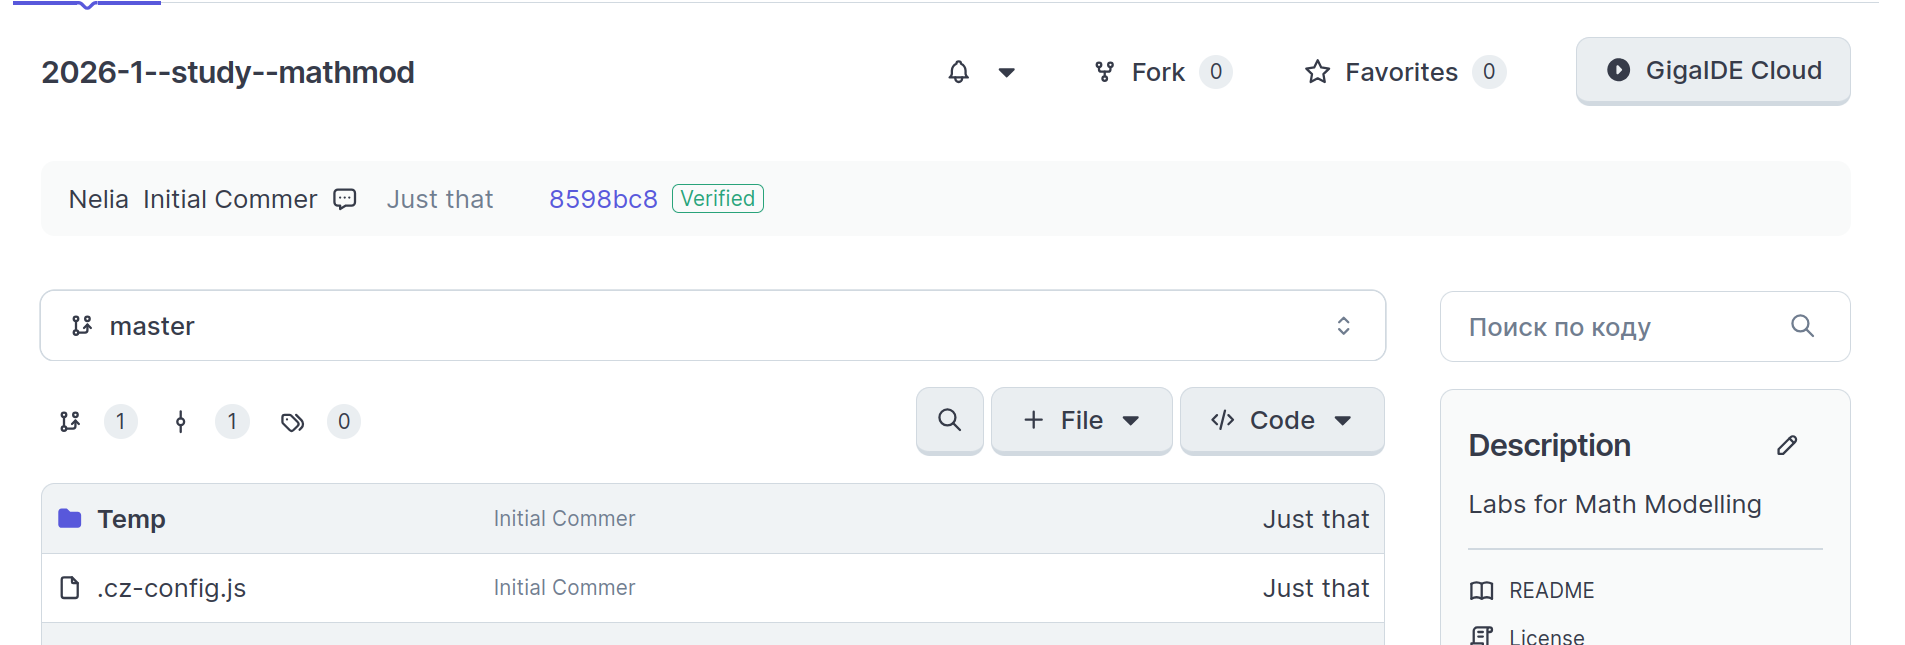
\includegraphics[width=0.7\textwidth,height=\textheight]{image/fig-035.png}

}

\caption{\label{fig-022}форматировка коммиты}

\end{figure}%

Я использую шаблон, указанный в руководстве, для создания нового
репозитория на gitverse(рис. 23)

\begin{figure}

\centering{

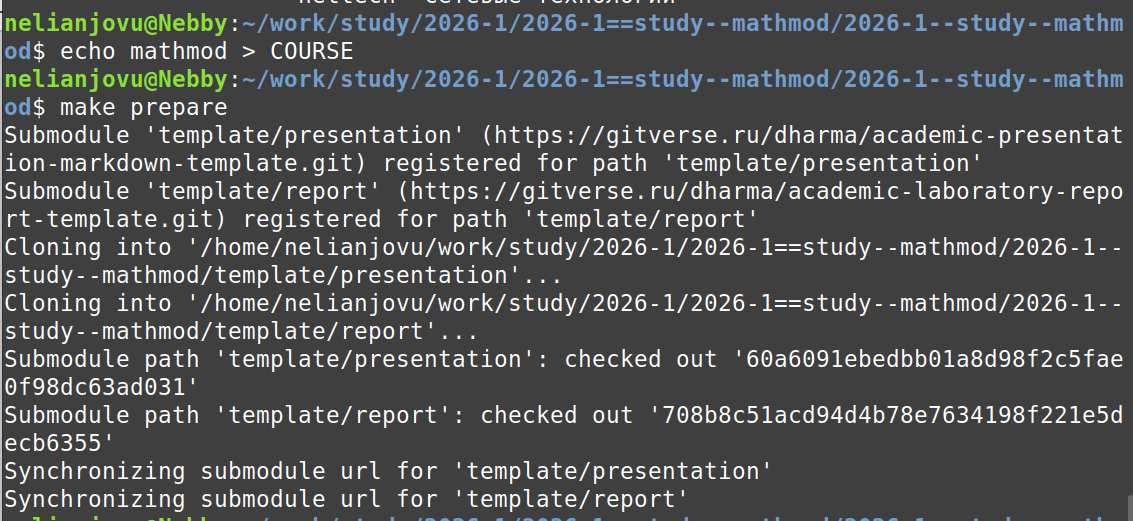
\includegraphics[width=0.7\textwidth,height=\textheight]{image/fig-038.png}

}

\caption{\label{fig-023}создание нового репозитория}

\end{figure}%

Я создаю файл для своей лабораторной работы, а затем клонирую
репозиторий(рис. 24)

\begin{figure}

\centering{

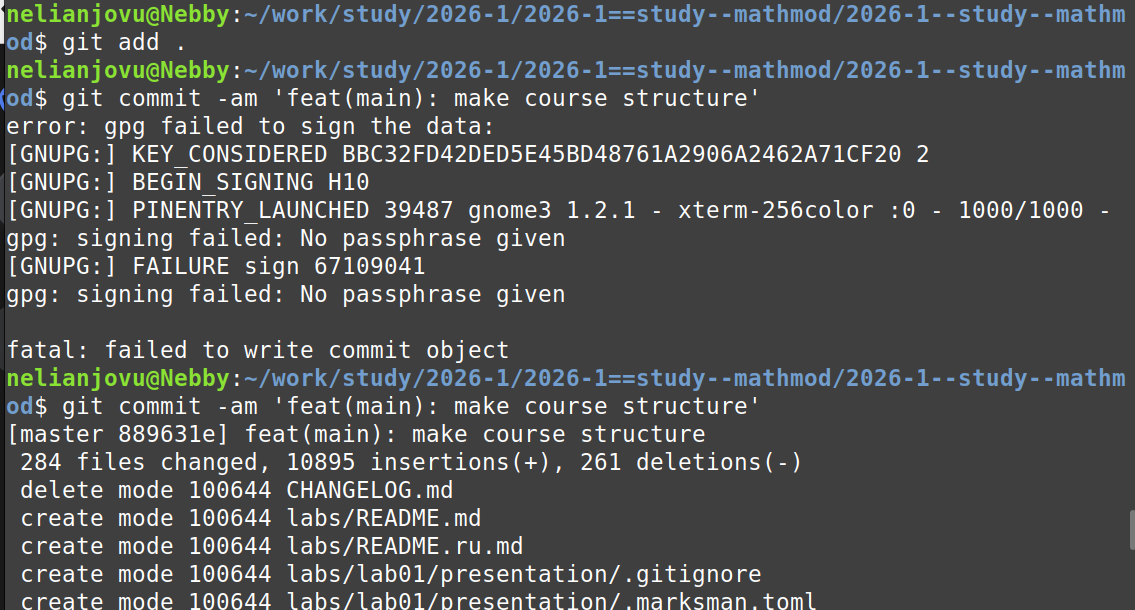
\includegraphics[width=0.7\textwidth,height=\textheight]{image/fig-039.png}

}

\caption{\label{fig-024}клонирование репозитория}

\end{figure}%

Я просматриваю доступные цели создания и список доступных курсов(рис.
25)

\begin{figure}

\centering{

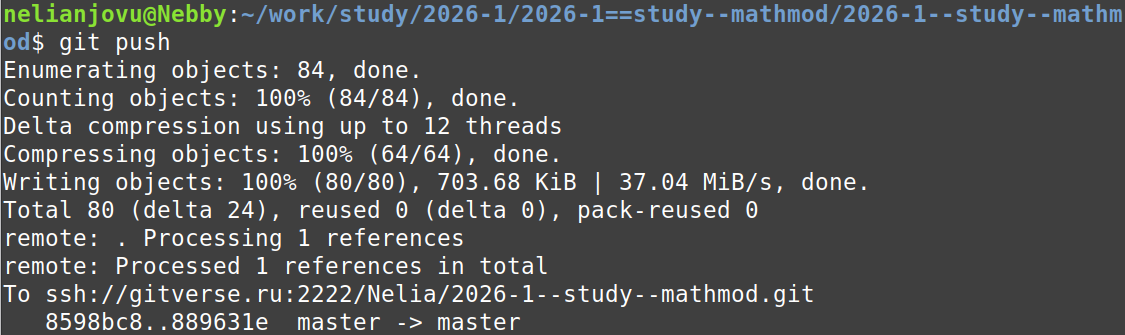
\includegraphics[width=0.7\textwidth,height=\textheight]{image/fig-040.png}

}

\caption{\label{fig-025}проверка доступных целей и списка курсов}

\end{figure}%

Я захожу в свой каталог лабораторных работ и инициализирую курс(рис. 26)

\begin{figure}

\centering{

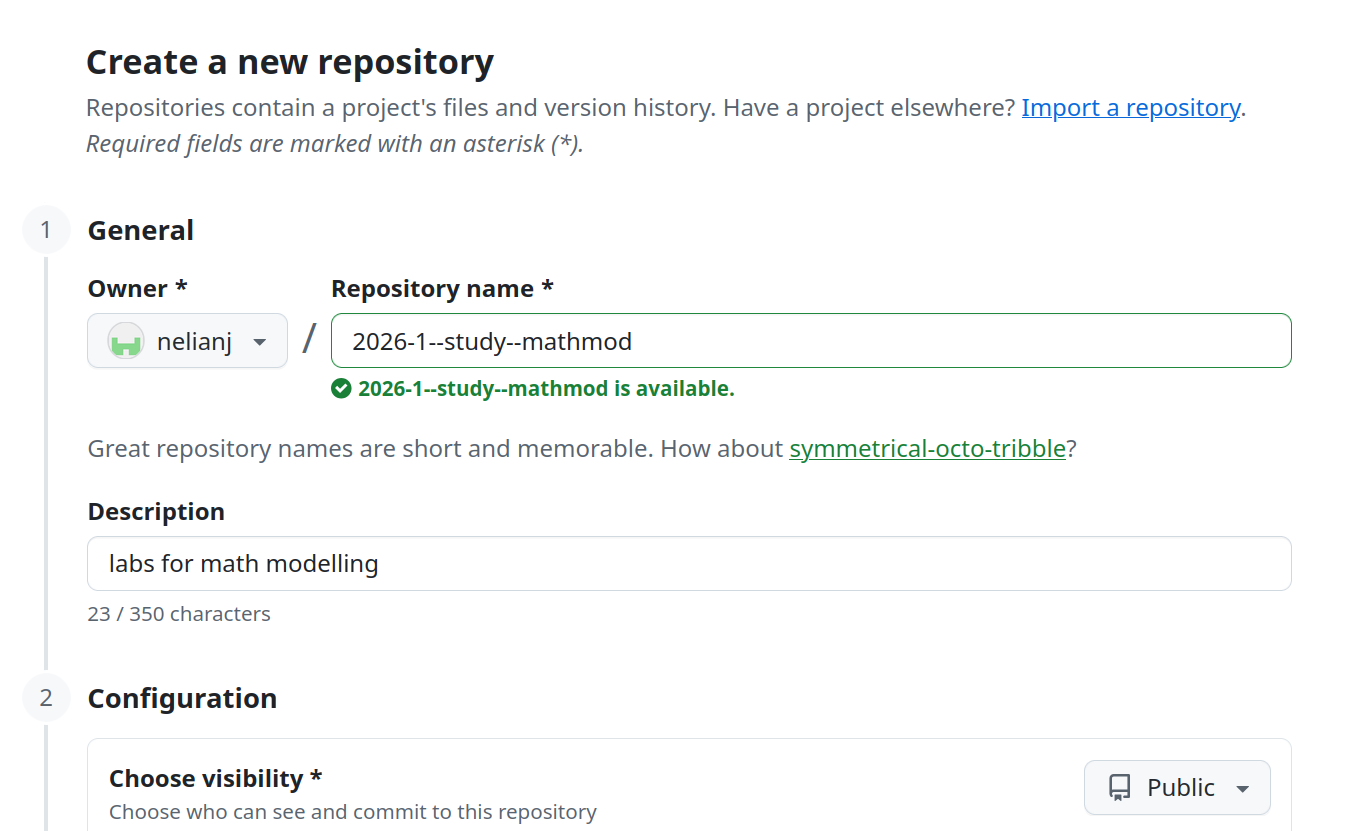
\includegraphics[width=0.7\textwidth,height=\textheight]{image/fig-041.png}

}

\caption{\label{fig-026}инициализация курса}

\end{figure}%

Я отправляю файлы на сервер(рис. 27)

\begin{figure}

\centering{

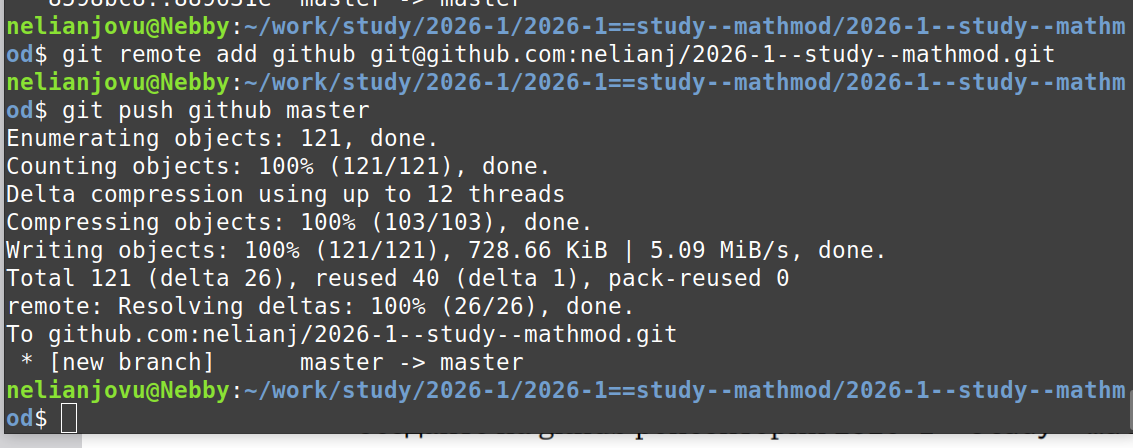
\includegraphics[width=0.7\textwidth,height=\textheight]{image/fig-042.png}

}

\caption{\label{fig-027}отправка файлов}

\end{figure}%

Я создаю репозиторий на github с именем 2026-1-study-mathmod(рис. 28)

\begin{figure}

\centering{

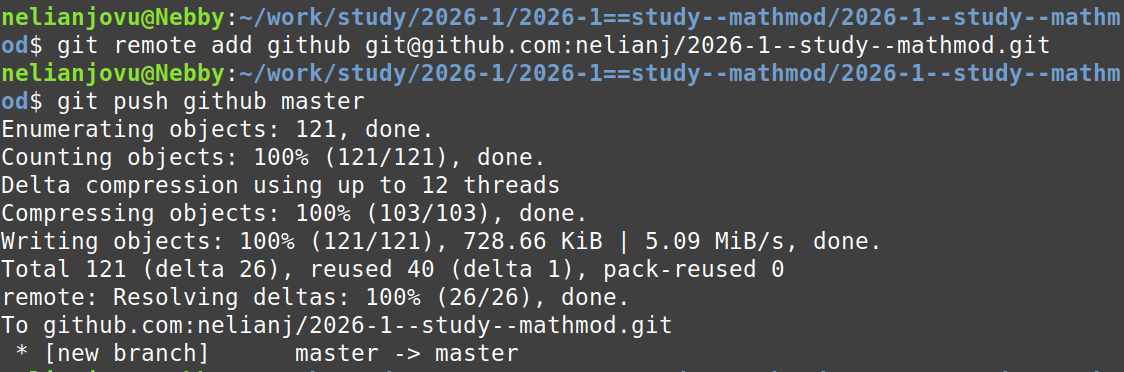
\includegraphics[width=0.7\textwidth,height=\textheight]{image/fig-044.png}

}

\caption{\label{fig-028}создание репозитория}

\end{figure}%

Я запускаю репозиторий на github(рис. 29)

\begin{figure}

\centering{

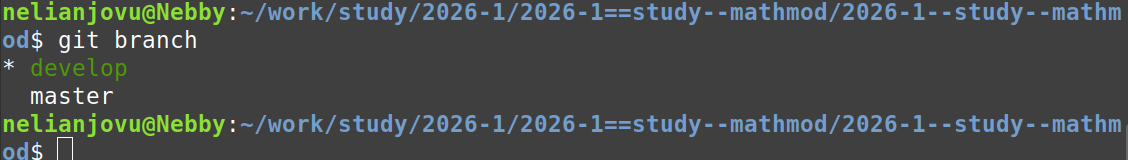
\includegraphics[width=0.7\textwidth,height=\textheight]{image/fig-045.png}

}

\caption{\label{fig-029}запуск репозитория}

\end{figure}%

Я инициализирую git flow и отвечаю на вопрос в соответствии с
инструкциями(рис. 30)

\begin{figure}

\centering{

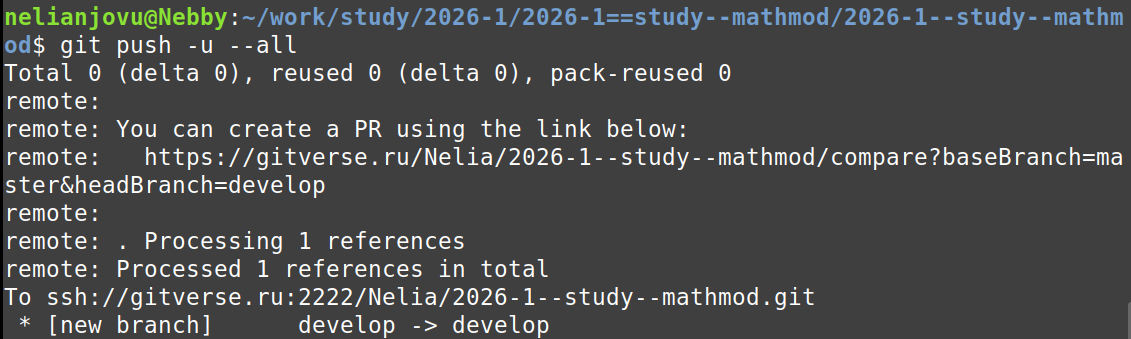
\includegraphics[width=0.7\textwidth,height=\textheight]{image/fig-046.png}

}

\caption{\label{fig-030}инициализация git flow}

\end{figure}%

Я проверяю и вижу, что нахожусь в ветке разработки. После чего загружаю
весь репозиторий на сервер(рис. 31)

\begin{figure}

\centering{

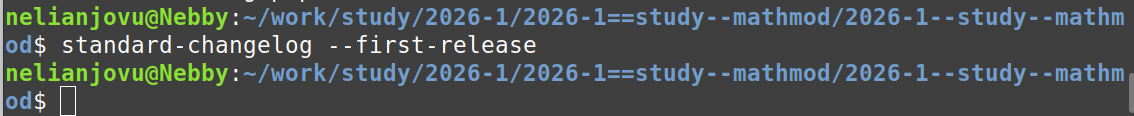
\includegraphics[width=0.7\textwidth,height=\textheight]{image/fig-048.png}

}

\caption{\label{fig-031}загрузка репозитория}

\end{figure}%

Я создаю релиз с версией 1.0.0 и создаю журнал изменений(рис. 32)

\begin{figure}

\centering{

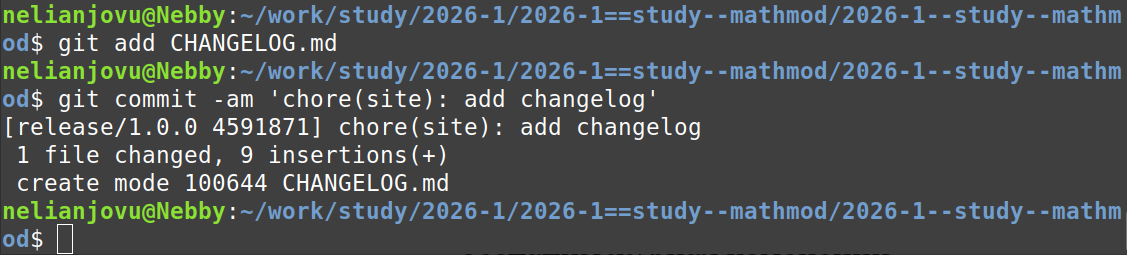
\includegraphics[width=0.7\textwidth,height=\textheight]{image/fig-049.png}

}

\caption{\label{fig-032}создание релиз}

\end{figure}%

Я добавляю журнал изменений в индекс и загружаю ветку выпуска в основную
ветку(рис. 33)

\begin{figure}

\centering{

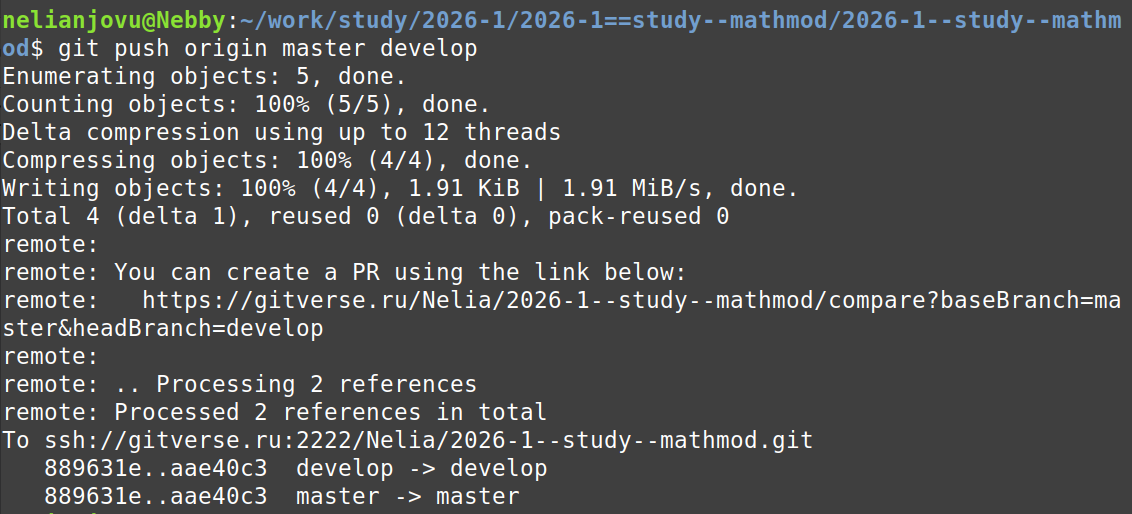
\includegraphics[width=0.7\textwidth,height=\textheight]{image/fig-051.png}

}

\caption{\label{fig-033}загрузка релиз}

\end{figure}%

После чего я отправляю данные на github(рис. 34)

\begin{figure}

\centering{

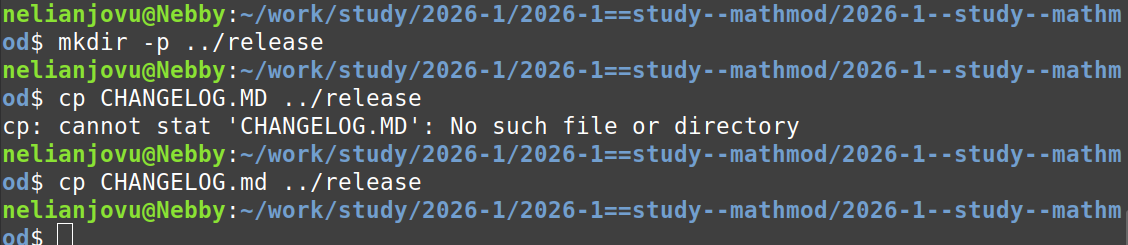
\includegraphics[width=0.7\textwidth,height=\textheight]{image/fig-053.png}

}

\caption{\label{fig-034}отправка данных}

\end{figure}%

Я копирую CHANGELOG.md в каталог релизов(рис. 35)

\begin{figure}

\centering{

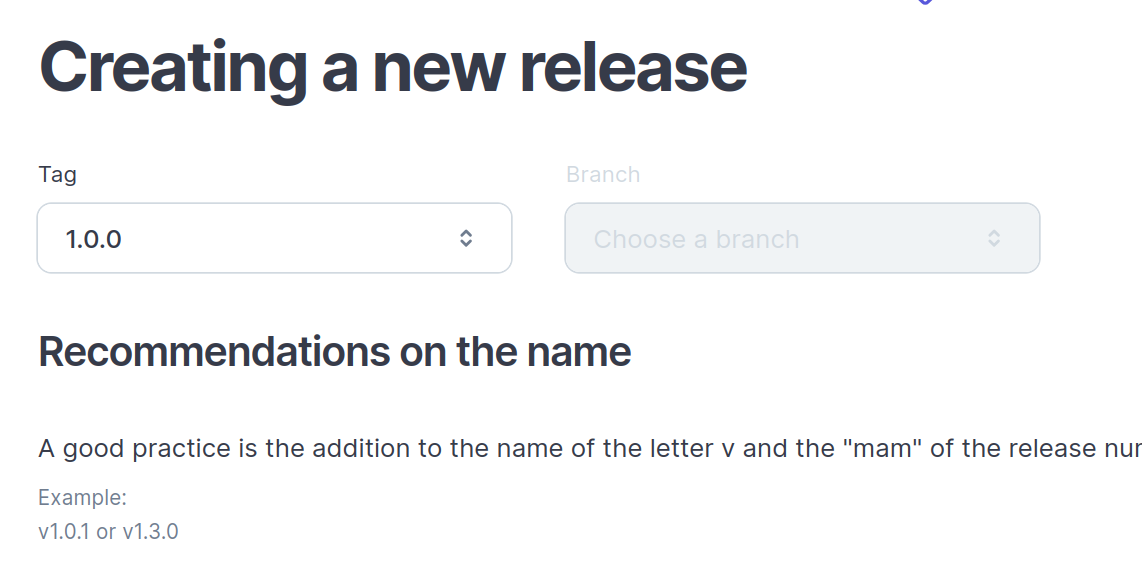
\includegraphics[width=0.7\textwidth,height=\textheight]{image/fig-054.png}

}

\caption{\label{fig-035}копирование файла}

\end{figure}%

Я создаю релиз вручную на gitverse(рис. 36)

\begin{figure}

\centering{

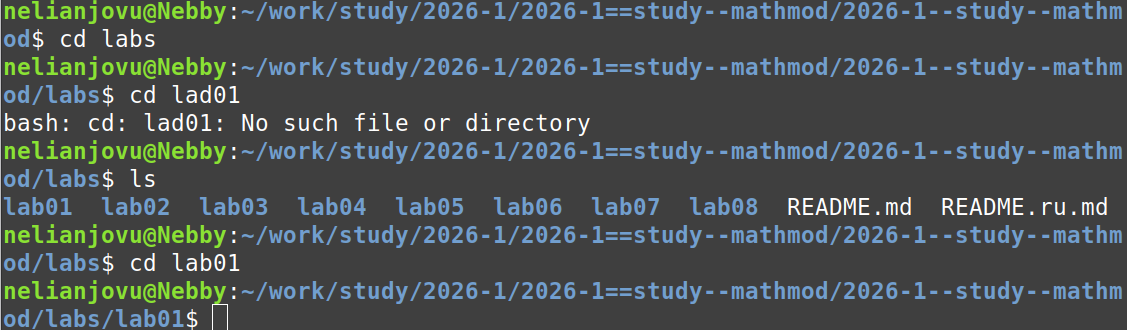
\includegraphics[width=0.7\textwidth,height=\textheight]{image/fig-055.png}

}

\caption{\label{fig-036}создание релиз}

\end{figure}%

\section{3. Создание проекта DrWatson для
лабораторных}\label{ux441ux43eux437ux434ux430ux43dux438ux435-ux43fux440ux43eux435ux43aux442ux430-drwatson-ux434ux43bux44f-ux43bux430ux431ux43eux440ux430ux442ux43eux440ux43dux44bux445}

Я захожу в каталог lab01, устанавливаю julia и запускаю его(рис. 37)

\begin{figure}

\centering{

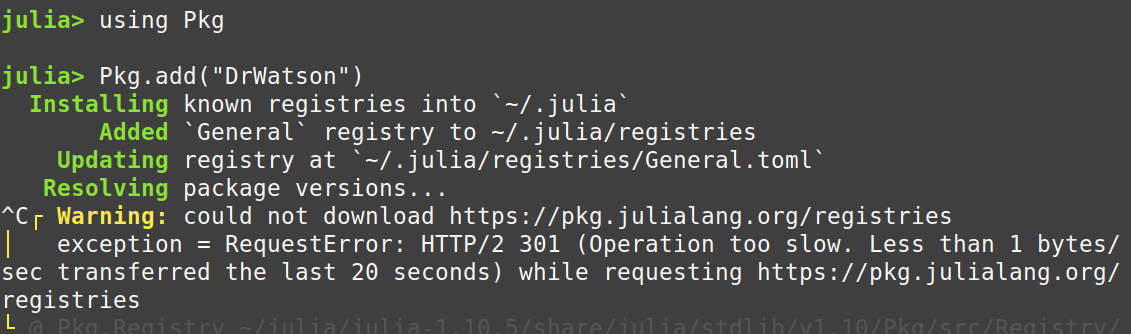
\includegraphics[width=0.7\textwidth,height=\textheight]{image/fig-057.png}

}

\caption{\label{fig-037}запуск julia}

\end{figure}%

Я создаю структуру проекта, используя пакет DrWatson в Julia's REPL(рис.
38)

\begin{figure}

\centering{

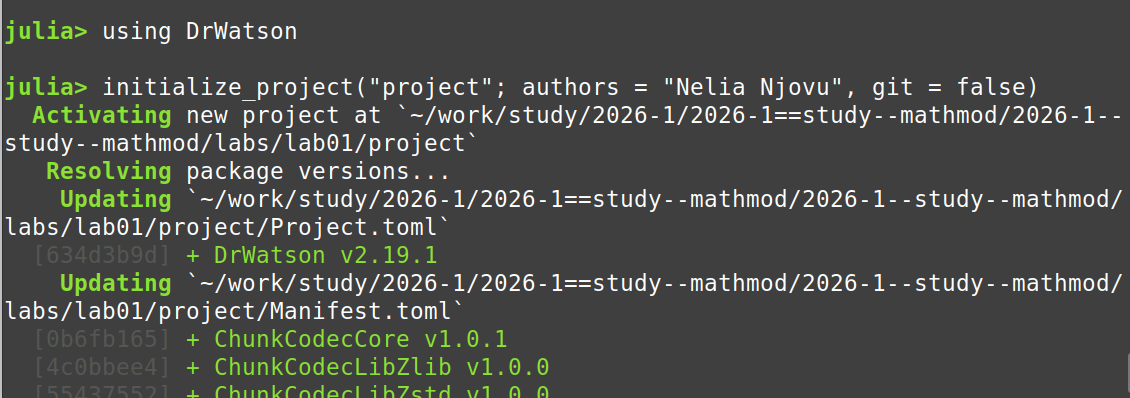
\includegraphics[width=0.7\textwidth,height=\textheight]{image/fig-058.png}

}

\caption{\label{fig-038}создание структуру}

\end{figure}%

Я создаю jl-файл, копирую и вставляю скрипт из руководства пользователя.
Скрипт настраивает всю структуру папок. После этого я запускаю файл(рис.
39)

\begin{figure}

\centering{

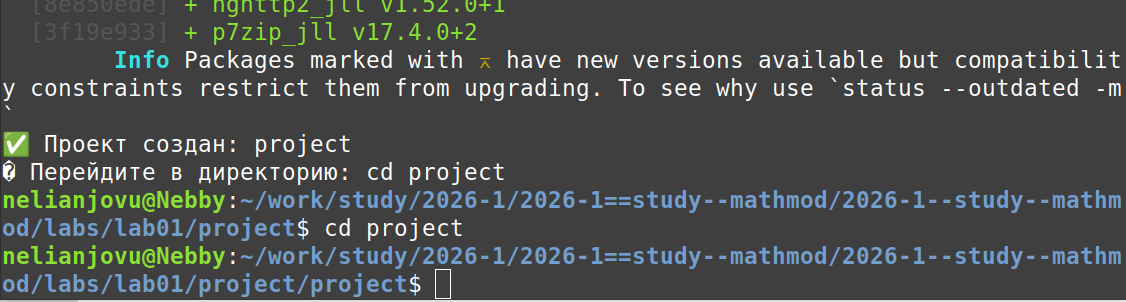
\includegraphics[width=0.7\textwidth,height=\textheight]{image/fig-060.png}

}

\caption{\label{fig-039a}создание первого jl-файла}

\end{figure}%

\begin{figure}

\centering{

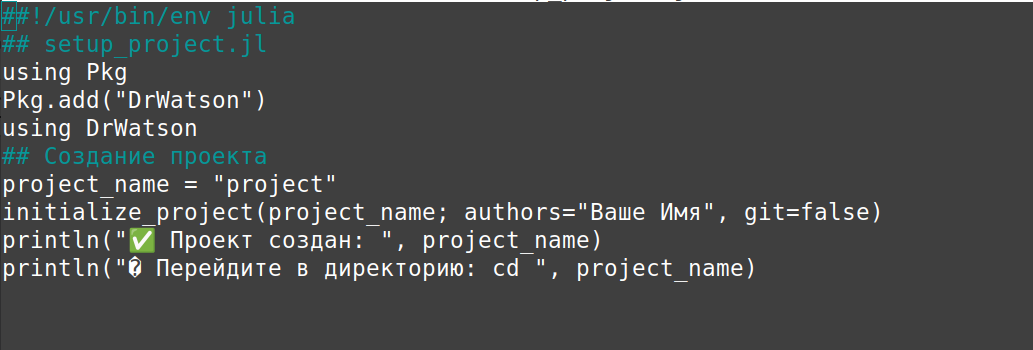
\includegraphics[width=0.7\textwidth,height=\textheight]{image/fig-061.png}

}

\caption{\label{fig-039b}создание первого jl-файла}

\end{figure}%

Я создаю jl-файл с именем add\_packages, копирую и вставляю скрипт из
руководства. Скрипт Этот скрипт устанавливает все пакеты Julia. После
этого я запускаю файл(рис. 40)

\begin{figure}

\centering{

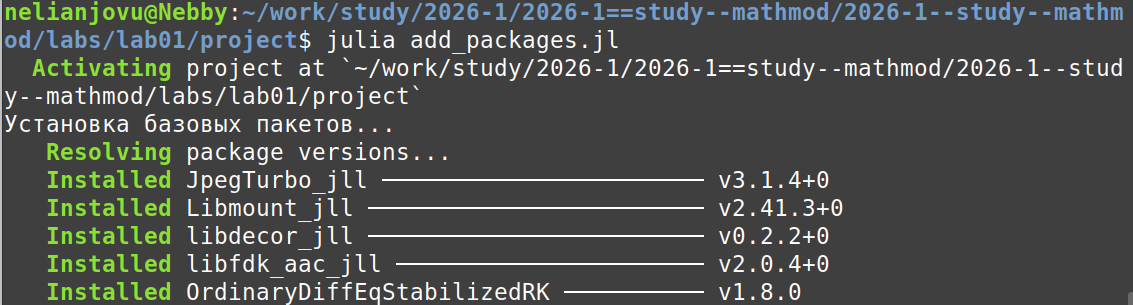
\includegraphics[width=0.7\textwidth,height=\textheight]{image/fig-063.png}

}

\caption{\label{fig-040}создание jl-файла add\_packages}

\end{figure}%

После установки я проверяю свою окончательную структуру проекта, и она
выглядит точно так же, как в руководстве(рис. 41)

\begin{figure}

\centering{

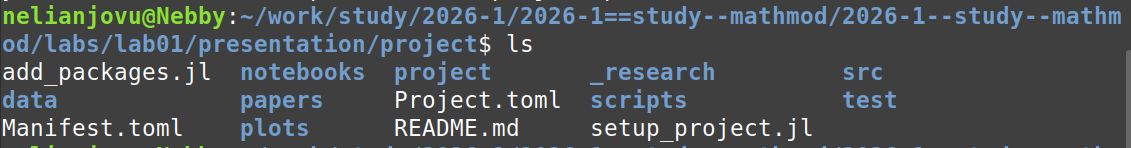
\includegraphics[width=0.7\textwidth,height=\textheight]{image/fig-066.png}

}

\caption{\label{fig-041}проверка структуру}

\end{figure}%

Я создаю jl-файл с именем 01\_exponential\_growth, копирую и вставляю
скрипт из руководства. Этот скрипт решает и визуализирует модель
экспоненциального роста(рис. 42)

\begin{figure}

\centering{

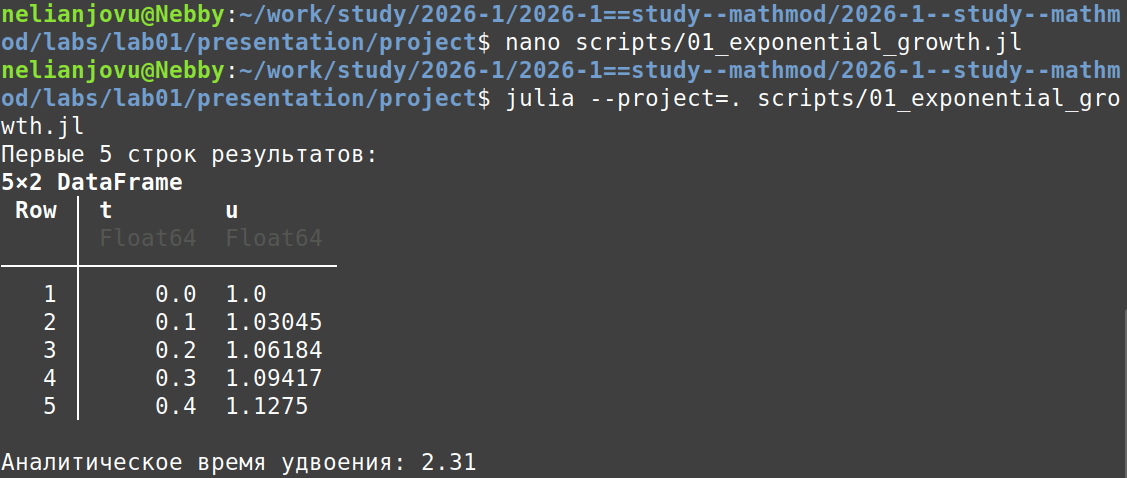
\includegraphics[width=0.7\textwidth,height=\textheight]{image/fig-068.png}

}

\caption{\label{fig-042}создание jl-файла 01\_exponential\_growth}

\end{figure}%

Полученные графики отображаются в каталоге plots(рис. 43)

\begin{figure}

\centering{

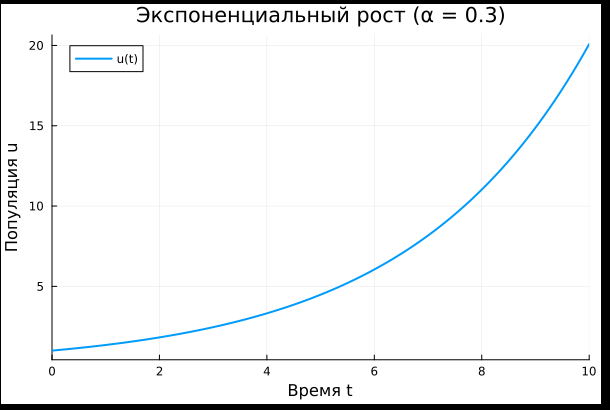
\includegraphics[width=0.7\textwidth,height=\textheight]{image/fig-069.png}

}

\caption{\label{fig-043}графики}

\end{figure}%

\section{4. Модель экспоненциального
роста}\label{ux43cux43eux434ux435ux43bux44c-ux44dux43aux441ux43fux43eux43dux435ux43dux446ux438ux430ux43bux44cux43dux43eux433ux43e-ux440ux43eux441ux442ux430}

Я редактирую скрипт в файле 01\_exponential\_growth. Новый скрипт
выполняет точно ту же математическую работу, что и предыдущий, за
исключением того, что теперь он написан в грамотном стиле
программирования(рис. 44)

!{[}отредактированный скрипт{]}(image/fig-070\{\#fig-044 width=70\%\}

Я создаю jl-файл с именем tangle, копирую и вставляю скрипт из
руководства. Этот скрипт представляет собой конвертер, который
использует файлы Julia literate (с комментариями и кодом) и
автоматически генерирует три разных формата: .jl; .qmd; .ipynb(рис. 45)

\begin{figure}

\centering{

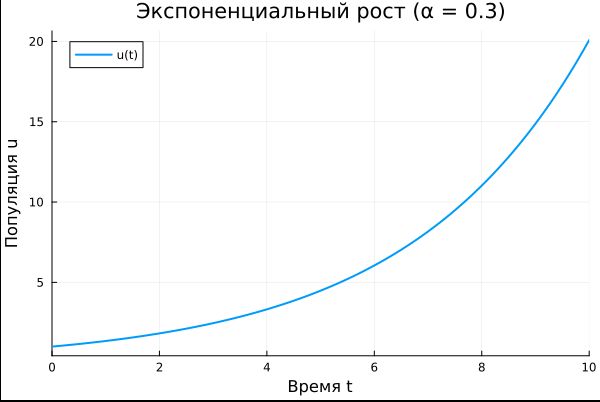
\includegraphics[width=0.7\textwidth,height=\textheight]{image/fig-072.png}

}

\caption{\label{fig-045}создание jl-файла tangle}

\end{figure}%

Я проверяю, был ли создан файл ipynb(рис. 46)

\begin{figure}

\centering{

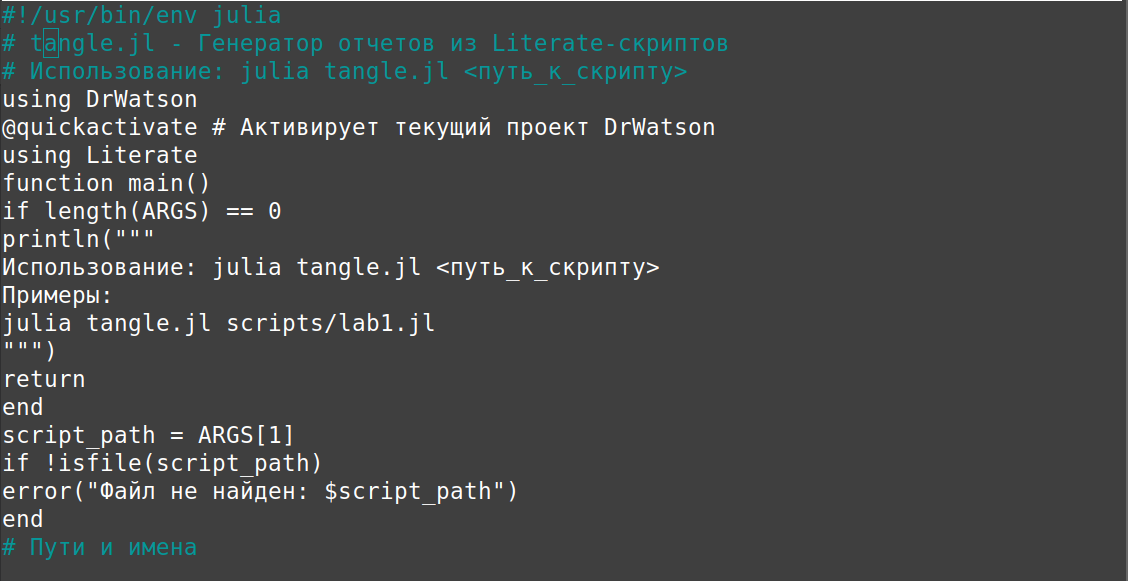
\includegraphics[width=0.7\textwidth,height=\textheight]{image/fig-073.png}

}

\caption{\label{fig-046}проверка файл}

\end{figure}%

В каталоге отчетов, в файле \_quarto.yml, я включаю поддержку кода
julia(рис. 47)

\begin{figure}

\centering{

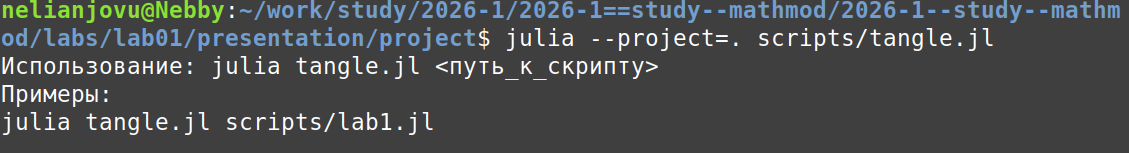
\includegraphics[width=0.7\textwidth,height=\textheight]{image/fig-075.png}

}

\caption{\label{fig-047}редактирование файла \_quarto.yml}

\end{figure}%

В преамбуле к preview.tex я подключаю пакет juliamono(рис. 48)

\begin{figure}

\centering{

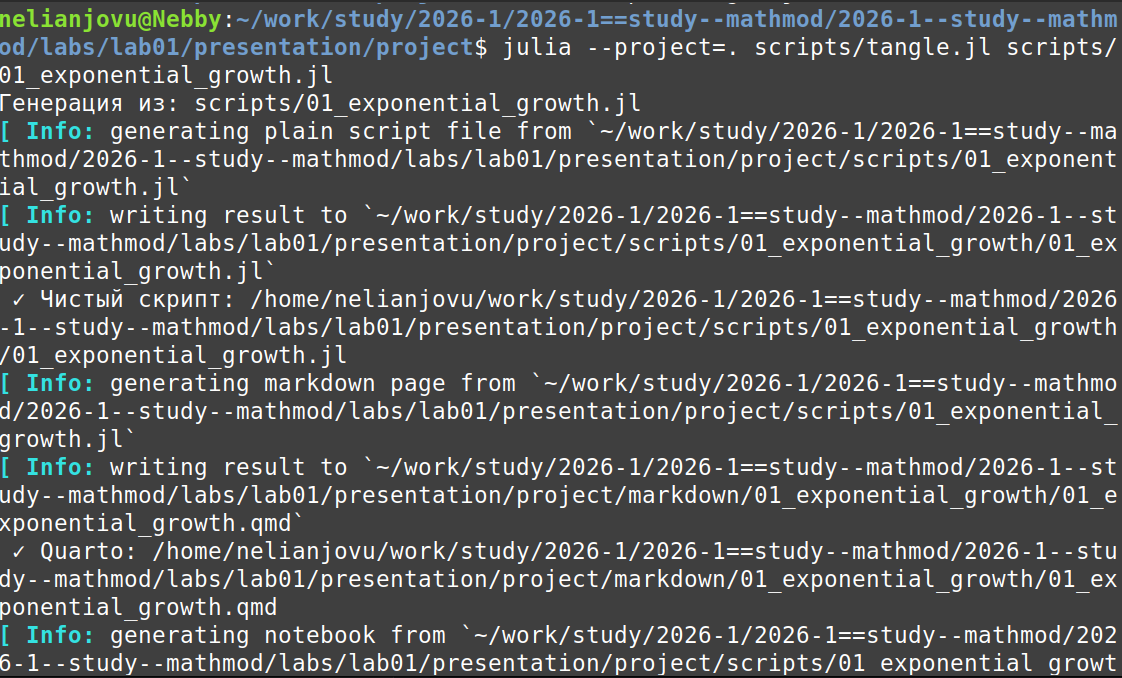
\includegraphics[width=0.7\textwidth,height=\textheight]{image/fig-076.png}

}

\caption{\label{fig-048}пакет juliamono}

\end{figure}%

\textbf{\emph{Ниже приведен код, результаты расчетов и графики для кода
в файле 01\_exponential\_growth.qmd}}

\chapter{Экспоненциальный
рост}\label{ux44dux43aux441ux43fux43eux43dux435ux43dux446ux438ux430ux43bux44cux43dux44bux439-ux440ux43eux441ux442}

\textbf{Цель:} Исследовать решение уравнения 𝑑𝑢/𝑑𝑡 = 𝛼𝑢.

\section{Инициализация проекта и загрузка
пакетов}\label{ux438ux43dux438ux446ux438ux430ux43bux438ux437ux430ux446ux438ux44f-ux43fux440ux43eux435ux43aux442ux430-ux438-ux437ux430ux433ux440ux443ux437ux43aux430-ux43fux430ux43aux435ux442ux43eux432}

\begin{Shaded}
\begin{Highlighting}[]
\ImportTok{using} \BuiltInTok{DrWatson}
\PreprocessorTok{@quickactivate} \StringTok{"project"}
\ImportTok{using} \BuiltInTok{DifferentialEquations}
\ImportTok{using} \BuiltInTok{Plots}
\CommentTok{\#force png format}
\FunctionTok{gr}\NormalTok{(size}\OperatorTok{=}\NormalTok{(}\FloatTok{800}\NormalTok{,}\FloatTok{600}\NormalTok{), fmt}\OperatorTok{=:}\NormalTok{png)}
\ImportTok{using} \BuiltInTok{DataFrames}
\ImportTok{using} \BuiltInTok{JLD2}
\NormalTok{script\_name }\OperatorTok{=} \FunctionTok{splitext}\NormalTok{(}\FunctionTok{basename}\NormalTok{(}\ConstantTok{PROGRAM\_FILE}\NormalTok{))[}\FloatTok{1}\NormalTok{]}
\FunctionTok{mkpath}\NormalTok{(}\FunctionTok{plotsdir}\NormalTok{(script\_name))}
\FunctionTok{mkpath}\NormalTok{(}\FunctionTok{datadir}\NormalTok{(script\_name))}
\end{Highlighting}
\end{Shaded}

\begin{verbatim}
┌ Warning: DrWatson could not find find a project file by recursively checking given `dir` and its parents. Returning `nothing` instead.
│ (given dir: /home/nelianjovu)
└ @ DrWatson ~/.julia/packages/DrWatson/2QF5p/src/project_setup.jl:84
\end{verbatim}

\begin{verbatim}
"/home/nelianjovu/work/study/2026-1/2026-1==study--mathmod/2026-1--study--mathmod/labs/lab01/project/data"
\end{verbatim}

\section{Определение
модели}\label{ux43eux43fux440ux435ux434ux435ux43bux435ux43dux438ux435-ux43cux43eux434ux435ux43bux438}

Уравнение экспоненциального роста: 𝑑𝑢/𝑑𝑡 = 𝛼𝑢, 𝑢(0) = 𝑢0

\begin{Shaded}
\begin{Highlighting}[]
\KeywordTok{function} \FunctionTok{exponential\_growth!}\NormalTok{(du, u, p, t)}
\NormalTok{α }\OperatorTok{=}\NormalTok{ p}
\NormalTok{du[}\FloatTok{1}\NormalTok{] }\OperatorTok{=}\NormalTok{ α }\OperatorTok{*}\NormalTok{ u[}\FloatTok{1}\NormalTok{]}
\KeywordTok{end}
\end{Highlighting}
\end{Shaded}

\begin{verbatim}
exponential_growth! (generic function with 1 method)
\end{verbatim}

\section{Первый запуск с параметрами по
умолчанию}\label{ux43fux435ux440ux432ux44bux439-ux437ux430ux43fux443ux441ux43a-ux441-ux43fux430ux440ux430ux43cux435ux442ux440ux430ux43cux438-ux43fux43e-ux443ux43cux43eux43bux447ux430ux43dux438ux44e}

Зададим начальные параметры:

\begin{Shaded}
\begin{Highlighting}[]
\NormalTok{u0 }\OperatorTok{=}\NormalTok{ [}\FloatTok{1.0}\NormalTok{] }\CommentTok{\# начальная популяция}
\NormalTok{α }\OperatorTok{=} \FloatTok{0.3} \CommentTok{\# скорость роста}
\NormalTok{tspan }\OperatorTok{=}\NormalTok{ (}\FloatTok{0.0}\NormalTok{, }\FloatTok{10.0}\NormalTok{) }\CommentTok{\# временной интервал}
\NormalTok{prob }\OperatorTok{=} \FunctionTok{ODEProblem}\NormalTok{(exponential\_growth!, u0, tspan, α)}
\NormalTok{sol }\OperatorTok{=} \FunctionTok{solve}\NormalTok{(prob, }\FunctionTok{Tsit5}\NormalTok{(), saveat}\OperatorTok{=}\FloatTok{0.1}\NormalTok{)}
\end{Highlighting}
\end{Shaded}

\begin{verbatim}
retcode: Success
Interpolation: 1st order linear
t: 101-element Vector{Float64}:
  0.0
  0.1
  0.2
  0.3
  0.4
  0.5
  0.6
  0.7
  0.8
  0.9
  1.0
  1.1
  1.2
  ⋮
  8.9
  9.0
  9.1
  9.2
  9.3
  9.4
  9.5
  9.6
  9.7
  9.8
  9.9
 10.0
u: 101-element Vector{Vector{Float64}}:
 [1.0]
 [1.030454533950446]
 [1.0618365551529674]
 [1.09417430287941]
 [1.1274968605386673]
 [1.161834232745065]
 [1.197217347699063]
 [1.2336780571872568]
 [1.2712491879500347]
 [1.3099646073864084]
 [1.349859018827382]
 [1.3909682733549678]
 [1.433329396499376]
 ⋮
 [14.439892233074882]
 [14.879627505035817]
 [15.332755966505253]
 [15.799688704153079]
 [16.280848966976613]
 [16.776672166300525]
 [17.287605875776944]
 [17.814109831385306]
 [18.356655931432517]
 [18.91572823655281]
 [19.491822969707833]
 [20.085448516186737]
\end{verbatim}

\section{Визуализация
результатов}\label{ux432ux438ux437ux443ux430ux43bux438ux437ux430ux446ux438ux44f-ux440ux435ux437ux443ux43bux44cux442ux430ux442ux43eux432}

Построим график решения:

\begin{Shaded}
\begin{Highlighting}[]
\FunctionTok{plot}\NormalTok{(sol, label}\OperatorTok{=}\StringTok{"u(t)"}\NormalTok{, xlabel}\OperatorTok{=}\StringTok{"Время t"}\NormalTok{, ylabel}\OperatorTok{=}\StringTok{"Популяция u"}\NormalTok{,}
\NormalTok{title}\OperatorTok{=}\StringTok{"Экспоненциальный рост (α = }\SpecialCharTok{$}\StringTok{α)", }\NormalTok{lw}\StringTok{=2, legend=:topleft)}
\end{Highlighting}
\end{Shaded}

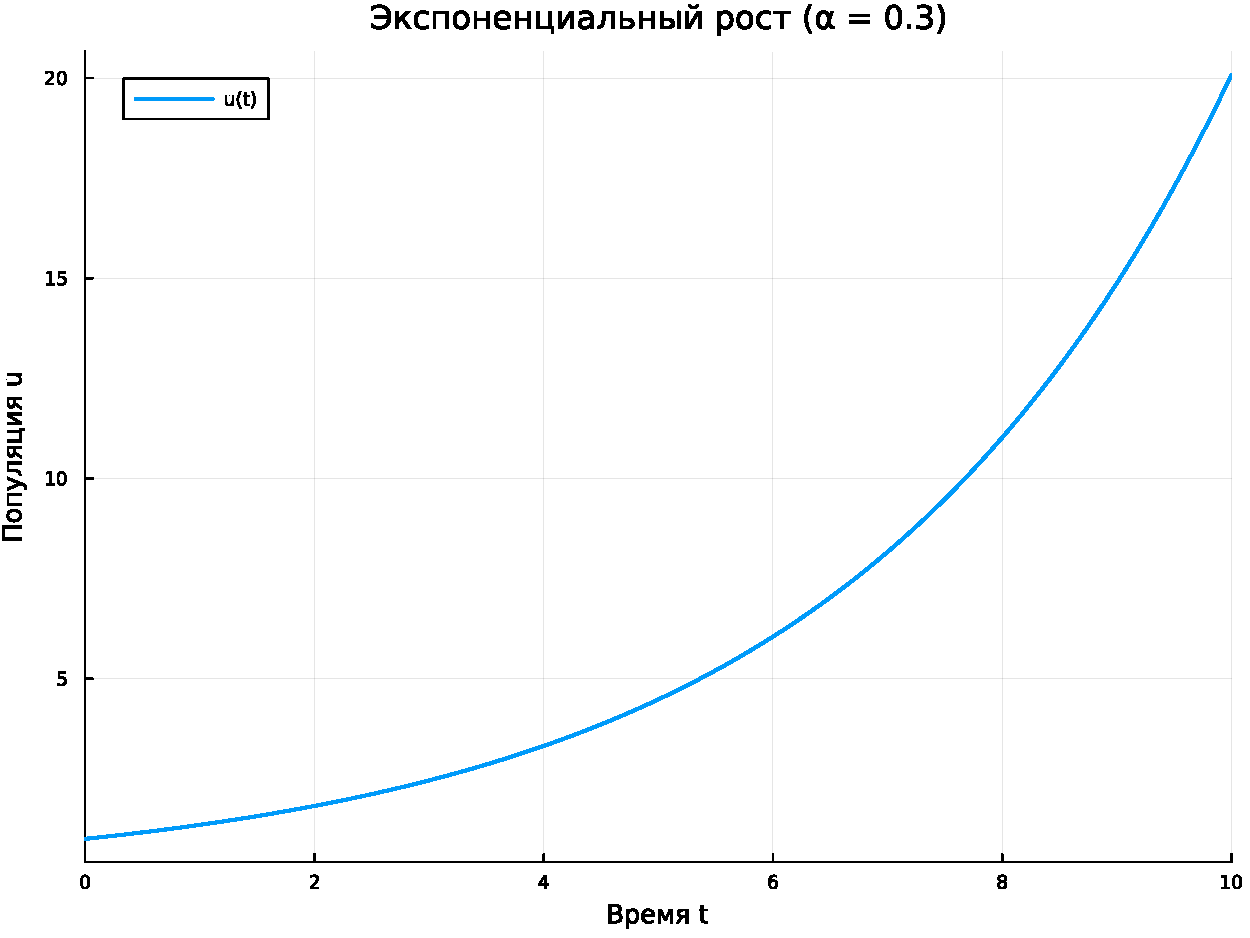
\includegraphics{mathmod-lab01-report-Nelia_files/mediabag/mathmod-lab01-report-Nelia_files/figure-pdf/cell-6-output-1.pdf}

Сохраним график в папку plots

\begin{Shaded}
\begin{Highlighting}[]
\FunctionTok{savefig}\NormalTok{(}\FunctionTok{plotsdir}\NormalTok{(script\_name, }\StringTok{"exponential\_growth\_α=}\SpecialCharTok{$}\StringTok{α.}\NormalTok{png}\StringTok{"}\NormalTok{))}
\end{Highlighting}
\end{Shaded}

\begin{verbatim}
"/home/nelianjovu/work/study/2026-1/2026-1==study--mathmod/2026-1--study--mathmod/labs/lab01/project/plots/exponential_growth_α=0.3.png"
\end{verbatim}

\section{Анализ
результатов}\label{ux430ux43dux430ux43bux438ux437-ux440ux435ux437ux443ux43bux44cux442ux430ux442ux43eux432}

Создадим таблицу с данными:

\begin{Shaded}
\begin{Highlighting}[]
\NormalTok{df }\OperatorTok{=} \FunctionTok{DataFrame}\NormalTok{(t}\OperatorTok{=}\NormalTok{sol.t, u}\OperatorTok{=}\FunctionTok{first}\NormalTok{.(sol.u))}
\FunctionTok{println}\NormalTok{(}\StringTok{"Первые 5 строк результатов:"}\NormalTok{)}
\FunctionTok{println}\NormalTok{(}\FunctionTok{first}\NormalTok{(df, }\FloatTok{5}\NormalTok{))}
\end{Highlighting}
\end{Shaded}

\begin{verbatim}
Первые 5 строк результатов:
5×2 DataFrame
 Row │ t        u       
     │ Float64  Float64 
─────┼──────────────────
   1 │     0.0  1.0
   2 │     0.1  1.03045
   3 │     0.2  1.06184
   4 │     0.3  1.09417
   5 │     0.4  1.1275
\end{verbatim}

Вычислим удвоение популяции:

\begin{Shaded}
\begin{Highlighting}[]
\NormalTok{u\_final }\OperatorTok{=} \FunctionTok{last}\NormalTok{(sol.u)[}\FloatTok{1}\NormalTok{]}
\NormalTok{doubling\_time }\OperatorTok{=} \FunctionTok{log}\NormalTok{(}\FloatTok{2}\NormalTok{) }\OperatorTok{/}\NormalTok{ α}
\FunctionTok{println}\NormalTok{(}\StringTok{"}\SpecialCharTok{\textbackslash{}n}\StringTok{Аналитическое время удвоения: "}\NormalTok{, }\FunctionTok{round}\NormalTok{(doubling\_time;digits}\OperatorTok{=}\FloatTok{2}\NormalTok{))}
\end{Highlighting}
\end{Shaded}

\begin{verbatim}

Аналитическое время удвоения: 2.31
\end{verbatim}

\section{Сохранение всех
результатов}\label{ux441ux43eux445ux440ux430ux43dux435ux43dux438ux435-ux432ux441ux435ux445-ux440ux435ux437ux443ux43bux44cux442ux430ux442ux43eux432}

\begin{Shaded}
\begin{Highlighting}[]
\PreprocessorTok{@save} \FunctionTok{datadir}\NormalTok{(script\_name, }\StringTok{"all\_results.jld2"}\NormalTok{) df}
\end{Highlighting}
\end{Shaded}

Я создаю jl-файл с именем 02\_exponential\_growth, копирую и вставляю
скрипт из руководства. Этот скрипт основан на предыдущей версии, но
добавляет систематическую проверку параметров и сравнительный анализ
производительности(рис. 49)

\begin{figure}

\centering{

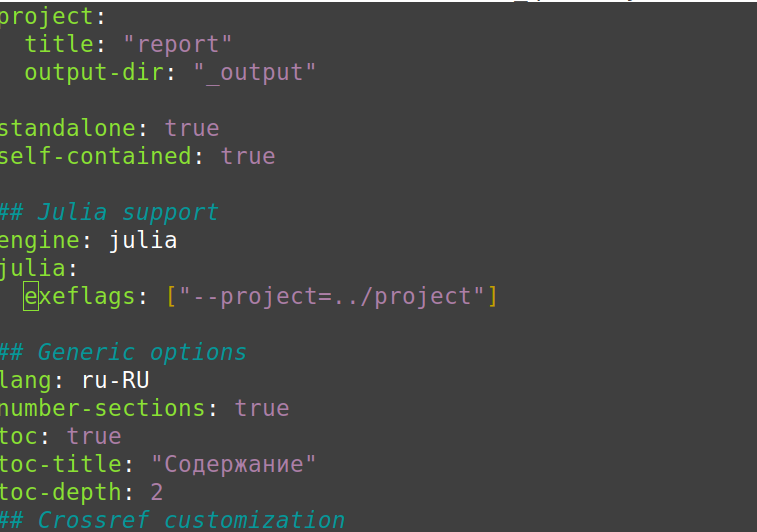
\includegraphics[width=0.7\textwidth,height=\textheight]{image/fig-079.png}

}

\caption{\label{fig-049}создание jl-файла 02\_exponential\_growth}

\end{figure}%

Используя tangle, я создаю три новых файла и открываю файл ipynb, чтобы
проверить его(рис. 50)

\begin{figure}

\centering{

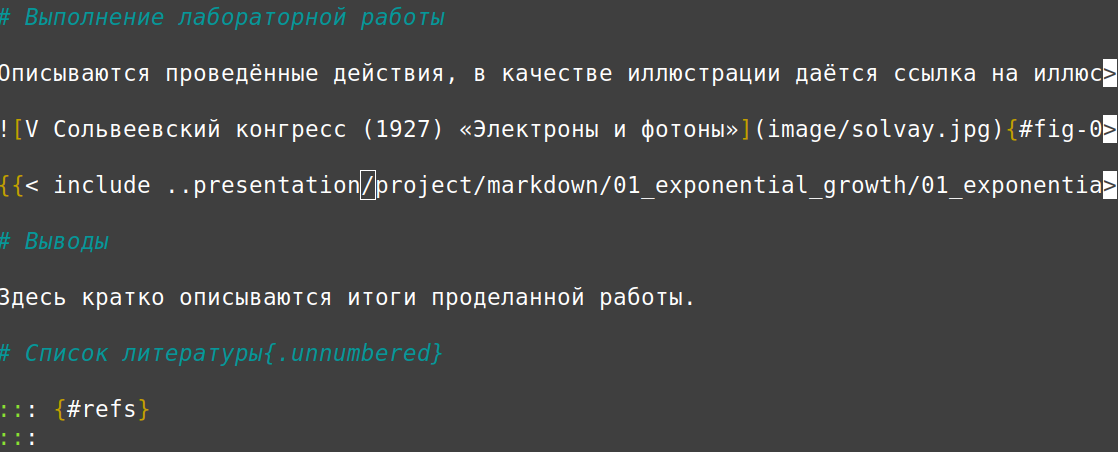
\includegraphics[width=0.7\textwidth,height=\textheight]{image/fig-081.png}

}

\caption{\label{fig-050}создание новых файлов}

\end{figure}%

\textbf{\emph{Ниже приведен код, результаты расчетов и графики для кода
в файле 02\_exponential\_growth.qmd}}

\chapter{Параметрическое исследование экспоненциального
роста}\label{ux43fux430ux440ux430ux43cux435ux442ux440ux438ux447ux435ux441ux43aux43eux435-ux438ux441ux441ux43bux435ux434ux43eux432ux430ux43dux438ux435-ux44dux43aux441ux43fux43eux43dux435ux43dux446ux438ux430ux43bux44cux43dux43eux433ux43e-ux440ux43eux441ux442ux430}

\section{Активация проекта и загрузка
пакетов}\label{ux430ux43aux442ux438ux432ux430ux446ux438ux44f-ux43fux440ux43eux435ux43aux442ux430-ux438-ux437ux430ux433ux440ux443ux437ux43aux430-ux43fux430ux43aux435ux442ux43eux432}

\textbf{ИЗМЕНЕНИЕ:} Добавлен DrWatson для управления проектом и
параметрами

\begin{Shaded}
\begin{Highlighting}[]
\ImportTok{using} \BuiltInTok{DrWatson}
\PreprocessorTok{@quickactivate} \StringTok{"project"}
\ImportTok{using} \BuiltInTok{DifferentialEquations}
\ImportTok{using} \BuiltInTok{DataFrames}
\ImportTok{using} \BuiltInTok{Plots}
\ImportTok{using} \BuiltInTok{JLD2}
\ImportTok{using} \BuiltInTok{BenchmarkTools}
\end{Highlighting}
\end{Shaded}

\begin{verbatim}
┌ Warning: DrWatson could not find find a project file by recursively checking given `dir` and its parents. Returning `nothing` instead.
│ (given dir: /home/nelianjovu)
└ @ DrWatson ~/.julia/packages/DrWatson/2QF5p/src/project_setup.jl:84
\end{verbatim}

Установка каталогов

\begin{Shaded}
\begin{Highlighting}[]
\NormalTok{script\_name }\OperatorTok{=} \FunctionTok{splitext}\NormalTok{(}\FunctionTok{basename}\NormalTok{(}\ConstantTok{PROGRAM\_FILE}\NormalTok{))[}\FloatTok{1}\NormalTok{]}
\FunctionTok{mkpath}\NormalTok{(}\FunctionTok{plotsdir}\NormalTok{(script\_name))}
\FunctionTok{mkpath}\NormalTok{(}\FunctionTok{datadir}\NormalTok{(script\_name))}
\end{Highlighting}
\end{Shaded}

\begin{verbatim}
"/home/nelianjovu/work/study/2026-1/2026-1==study--mathmod/2026-1--study--mathmod/labs/lab01/project/data"
\end{verbatim}

\section{Определение
модели}\label{ux43eux43fux440ux435ux434ux435ux43bux435ux43dux438ux435-ux43cux43eux434ux435ux43bux438-1}

Модель: 𝑑𝑢/𝑑𝑡 = 𝛼 ⋅ 𝑢

\begin{Shaded}
\begin{Highlighting}[]
\KeywordTok{function} \FunctionTok{exponential\_growth!}\NormalTok{(du, u, p, t)}
\NormalTok{    α }\OperatorTok{=}\NormalTok{ p.α}
\NormalTok{    du[}\FloatTok{1}\NormalTok{] }\OperatorTok{=}\NormalTok{ α }\OperatorTok{*}\NormalTok{ u[}\FloatTok{1}\NormalTok{]}
\KeywordTok{end}
\end{Highlighting}
\end{Shaded}

\begin{verbatim}
exponential_growth! (generic function with 1 method)
\end{verbatim}

\section{Определение параметров в
Dict}\label{ux43eux43fux440ux435ux434ux435ux43bux435ux43dux438ux435-ux43fux430ux440ux430ux43cux435ux442ux440ux43eux432-ux432-dict}

\textbf{ОСНОВНОЕ ИЗМЕНЕНИЕ:} Все параметры собраны в Dict для
систематизации

Базовый набор параметров (один эксперимент)

\begin{Shaded}
\begin{Highlighting}[]
\NormalTok{base\_params }\OperatorTok{=} \FunctionTok{Dict}\NormalTok{(}
    \OperatorTok{:}\NormalTok{u0 }\OperatorTok{=\textgreater{}}\NormalTok{ [}\FloatTok{1.0}\NormalTok{],}
    \OperatorTok{:}\NormalTok{α }\OperatorTok{=\textgreater{}} \FloatTok{0.3}\NormalTok{,}
    \OperatorTok{:}\NormalTok{tspan }\OperatorTok{=\textgreater{}}\NormalTok{ (}\FloatTok{0.0}\NormalTok{, }\FloatTok{10.0}\NormalTok{),}
    \OperatorTok{:}\NormalTok{solver }\OperatorTok{=\textgreater{}} \FunctionTok{Tsit5}\NormalTok{(),}
    \OperatorTok{:}\NormalTok{saveat }\OperatorTok{=\textgreater{}} \FloatTok{0.1}\NormalTok{,}
    \OperatorTok{:}\NormalTok{experiment\_name }\OperatorTok{=\textgreater{}} \StringTok{"base\_experiment"}
\NormalTok{)}

\FunctionTok{println}\NormalTok{(}\StringTok{"Базовые параметры эксперимента:"}\NormalTok{)}
\ControlFlowTok{for}\NormalTok{ (key, value) }\KeywordTok{in}\NormalTok{ base\_params}
    \FunctionTok{println}\NormalTok{(}\StringTok{" }\SpecialCharTok{$}\NormalTok{key}\StringTok{ = }\SpecialCharTok{$}\NormalTok{value}\StringTok{"}\NormalTok{)}
\ControlFlowTok{end}
\end{Highlighting}
\end{Shaded}

\begin{verbatim}
Базовые параметры эксперимента:
 α = 0.3
 u0 = [1.0]
 saveat = 0.1
 solver = Tsit5{typeof(OrdinaryDiffEqCore.trivial_limiter!), typeof(OrdinaryDiffEqCore.trivial_limiter!), Static.False}(OrdinaryDiffEqCore.trivial_limiter!, OrdinaryDiffEqCore.trivial_limiter!, static(false))
 experiment_name = base_experiment
 tspan = (0.0, 10.0)
\end{verbatim}

\section{Функция-обертка для запуска одного
эксперимента}\label{ux444ux443ux43dux43aux446ux438ux44f-ux43eux431ux435ux440ux442ux43aux430-ux434ux43bux44f-ux437ux430ux43fux443ux441ux43aux430-ux43eux434ux43dux43eux433ux43e-ux44dux43aux441ux43fux435ux440ux438ux43cux435ux43dux442ux430}

\textbf{ИСПРАВЛЕНИЕ:} Возвращаем Dict со строковыми ключами

\begin{Shaded}
\begin{Highlighting}[]
\KeywordTok{function} \FunctionTok{run\_single\_experiment}\NormalTok{(params}\OperatorTok{::}\DataTypeTok{Dict}\NormalTok{)}
    \PreprocessorTok{@unpack}\NormalTok{ u0, α, tspan, solver, saveat }\OperatorTok{=}\NormalTok{ params}
\NormalTok{    prob }\OperatorTok{=} \FunctionTok{ODEProblem}\NormalTok{(exponential\_growth!, u0, tspan, (α}\OperatorTok{=}\NormalTok{α,))}
\NormalTok{    sol }\OperatorTok{=} \FunctionTok{solve}\NormalTok{(prob, solver; saveat}\OperatorTok{=}\NormalTok{saveat)}
\NormalTok{    final\_population }\OperatorTok{=} \FunctionTok{last}\NormalTok{(sol.u)[}\FloatTok{1}\NormalTok{]}
\NormalTok{    doubling\_time }\OperatorTok{=} \FunctionTok{log}\NormalTok{(}\FloatTok{2}\NormalTok{) }\OperatorTok{/}\NormalTok{ α}
    \ControlFlowTok{return} \FunctionTok{Dict}\NormalTok{(}
        \StringTok{"solution"} \OperatorTok{=\textgreater{}}\NormalTok{ sol,}
        \StringTok{"time\_points"} \OperatorTok{=\textgreater{}}\NormalTok{ sol.t,}
        \StringTok{"population\_values"} \OperatorTok{=\textgreater{}} \FunctionTok{first}\NormalTok{.(sol.u),}
        \StringTok{"final\_population"} \OperatorTok{=\textgreater{}}\NormalTok{ final\_population,}
        \StringTok{"doubling\_time"} \OperatorTok{=\textgreater{}}\NormalTok{ doubling\_time,}
        \StringTok{"parameters"} \OperatorTok{=\textgreater{}}\NormalTok{ params}
\NormalTok{    )}
\KeywordTok{end}
\end{Highlighting}
\end{Shaded}

\begin{verbatim}
run_single_experiment (generic function with 1 method)
\end{verbatim}

\section{Запуск базового
эксперимента}\label{ux437ux430ux43fux443ux441ux43a-ux431ux430ux437ux43eux432ux43eux433ux43e-ux44dux43aux441ux43fux435ux440ux438ux43cux435ux43dux442ux430}

\textbf{ИЗМЕНЕНИЕ:} Используем produce\_or\_load для автоматического
кэширования

\begin{Shaded}
\begin{Highlighting}[]
\NormalTok{data, path }\OperatorTok{=} \FunctionTok{produce\_or\_load}\NormalTok{(}
    \FunctionTok{datadir}\NormalTok{(script\_name, }\StringTok{"single"}\NormalTok{),}
\NormalTok{    base\_params,}
\NormalTok{    run\_single\_experiment,}
\NormalTok{    prefix }\OperatorTok{=} \StringTok{"exp\_growth"}\NormalTok{,}
\NormalTok{    tag }\OperatorTok{=} \ConstantTok{false}\NormalTok{,}
\NormalTok{    verbose }\OperatorTok{=} \ConstantTok{true}
\NormalTok{)}

\FunctionTok{println}\NormalTok{(}\StringTok{"}\SpecialCharTok{\textbackslash{}n}\StringTok{Результаты базового эксперимента:"}\NormalTok{)}
\FunctionTok{println}\NormalTok{(}\StringTok{" Финальная популяция: "}\NormalTok{, data[}\StringTok{"final\_population"}\NormalTok{])}
\FunctionTok{println}\NormalTok{(}\StringTok{" Время удвоения: "}\NormalTok{, }\FunctionTok{round}\NormalTok{(data[}\StringTok{"doubling\_time"}\NormalTok{], digits}\OperatorTok{=}\FloatTok{2}\NormalTok{))}
\FunctionTok{println}\NormalTok{(}\StringTok{" Файл результатов: "}\NormalTok{, path)}
\end{Highlighting}
\end{Shaded}

\begin{verbatim}

Результаты базового эксперимента:
 Финальная популяция: 20.085448516186737
 Время удвоения: 2.31
 Файл результатов: /home/nelianjovu/work/study/2026-1/2026-1==study--mathmod/2026-1--study--mathmod/labs/lab01/project/data/single/exp_growth_experiment_name=base_experiment_saveat=0.1_α=0.3.jld2
\end{verbatim}

\section{Визуализация базового
эксперимента}\label{ux432ux438ux437ux443ux430ux43bux438ux437ux430ux446ux438ux44f-ux431ux430ux437ux43eux432ux43eux433ux43e-ux44dux43aux441ux43fux435ux440ux438ux43cux435ux43dux442ux430}

\begin{Shaded}
\begin{Highlighting}[]
\NormalTok{p1 }\OperatorTok{=} \FunctionTok{plot}\NormalTok{(data[}\StringTok{"time\_points"}\NormalTok{], data[}\StringTok{"population\_values"}\NormalTok{],}
\NormalTok{    label}\OperatorTok{=}\StringTok{"α = }\SpecialCharTok{$}\NormalTok{(base\_params[}\OperatorTok{:}\NormalTok{α])}\StringTok{"}\NormalTok{,}
\NormalTok{    xlabel}\OperatorTok{=}\StringTok{"Время, t"}\NormalTok{,}
\NormalTok{    ylabel}\OperatorTok{=}\StringTok{"Популяция, u(t)"}\NormalTok{,}
\NormalTok{    title}\OperatorTok{=}\StringTok{"Экспоненциальный рост (базовый эксперимент)"}\NormalTok{,}
\NormalTok{    lw}\OperatorTok{=}\FloatTok{2}\NormalTok{,}
\NormalTok{    legend}\OperatorTok{=:}\NormalTok{topleft,}
\NormalTok{    grid}\OperatorTok{=}\ConstantTok{true}
\NormalTok{)}
\end{Highlighting}
\end{Shaded}

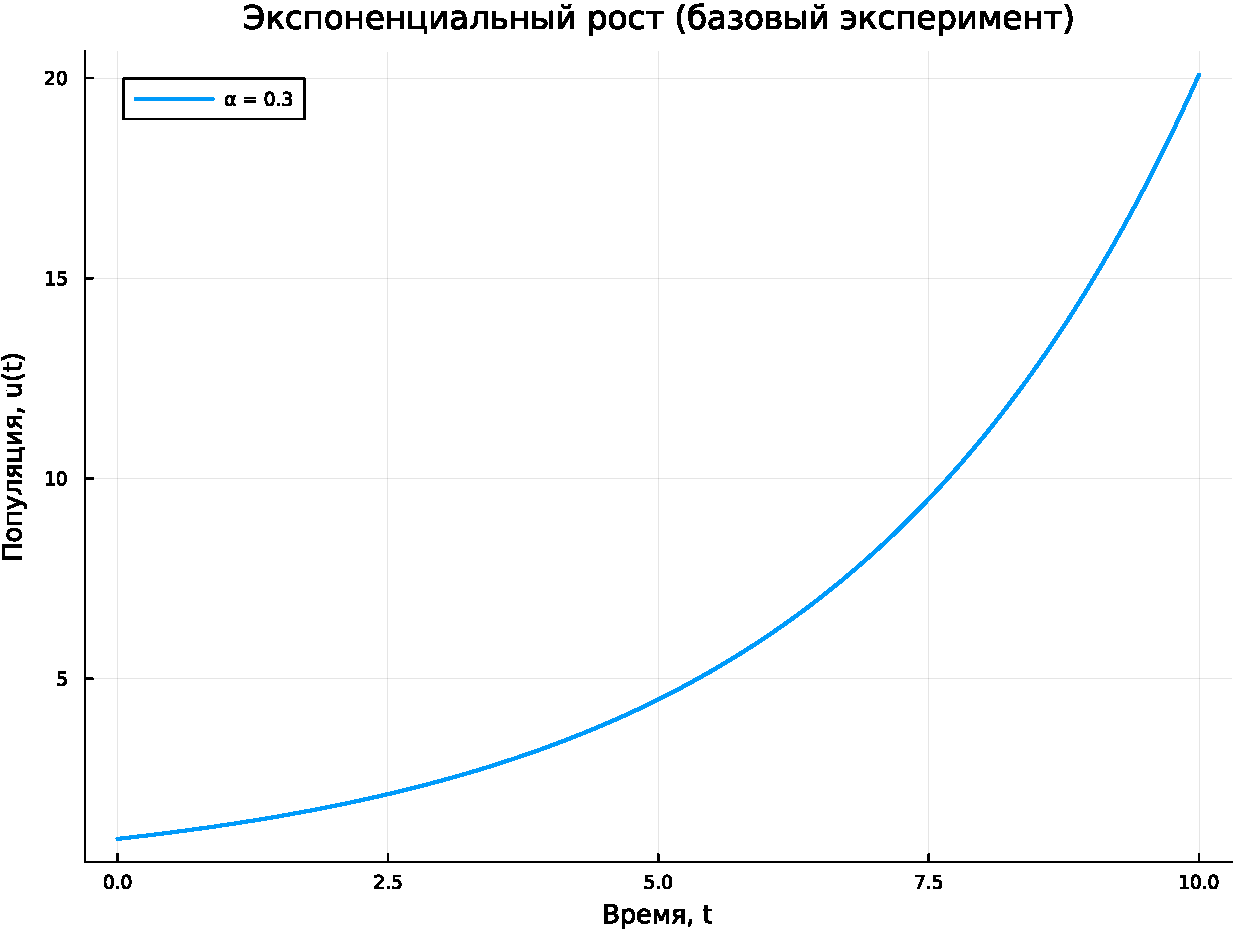
\includegraphics{mathmod-lab01-report-Nelia_files/mediabag/mathmod-lab01-report-Nelia_files/figure-pdf/cell-17-output-1.pdf}

Сохраним график в папку plots

\begin{Shaded}
\begin{Highlighting}[]
\FunctionTok{savefig}\NormalTok{(}\FunctionTok{plotsdir}\NormalTok{(script\_name, }\StringTok{"single\_experiment.png"}\NormalTok{))}
\end{Highlighting}
\end{Shaded}

\begin{verbatim}
"/home/nelianjovu/work/study/2026-1/2026-1==study--mathmod/2026-1--study--mathmod/labs/lab01/project/plots/single_experiment.png"
\end{verbatim}

\section{Параметрическое
сканирование}\label{ux43fux430ux440ux430ux43cux435ux442ux440ux438ux447ux435ux441ux43aux43eux435-ux441ux43aux430ux43dux438ux440ux43eux432ux430ux43dux438ux435}

\textbf{НОВАЯ СЕКЦИЯ:} Исследование влияния параметра α

Сетка параметров для сканирования

\begin{Shaded}
\begin{Highlighting}[]
\NormalTok{param\_grid }\OperatorTok{=} \FunctionTok{Dict}\NormalTok{(}
    \OperatorTok{:}\NormalTok{u0 }\OperatorTok{=\textgreater{}}\NormalTok{ [[}\FloatTok{1.0}\NormalTok{]],}
    \OperatorTok{:}\NormalTok{α }\OperatorTok{=\textgreater{}}\NormalTok{ [}\FloatTok{0.1}\NormalTok{, }\FloatTok{0.3}\NormalTok{, }\FloatTok{0.5}\NormalTok{, }\FloatTok{0.8}\NormalTok{, }\FloatTok{1.0}\NormalTok{],}
    \OperatorTok{:}\NormalTok{tspan }\OperatorTok{=\textgreater{}}\NormalTok{ [(}\FloatTok{0.0}\NormalTok{, }\FloatTok{10.0}\NormalTok{)],}
    \OperatorTok{:}\NormalTok{solver }\OperatorTok{=\textgreater{}}\NormalTok{ [}\FunctionTok{Tsit5}\NormalTok{()],}
    \OperatorTok{:}\NormalTok{saveat }\OperatorTok{=\textgreater{}}\NormalTok{ [}\FloatTok{0.1}\NormalTok{],}
    \OperatorTok{:}\NormalTok{experiment\_name }\OperatorTok{=\textgreater{}}\NormalTok{ [}\StringTok{"parametric\_scan"}\NormalTok{]}
\NormalTok{)}
\end{Highlighting}
\end{Shaded}

\begin{verbatim}
Dict{Symbol, Vector} with 6 entries:
  :α               => [0.1, 0.3, 0.5, 0.8, 1.0]
  :u0              => [[1.0]]
  :saveat          => [0.1]
  :solver          => [Tsit5{typeof(trivial_limiter!), typeof(trivial_limiter!)…
  :experiment_name => ["parametric_scan"]
  :tspan           => [(0.0, 10.0)]
\end{verbatim}

Генерация всех комбинаций параметров

\begin{Shaded}
\begin{Highlighting}[]
\NormalTok{all\_params }\OperatorTok{=} \FunctionTok{dict\_list}\NormalTok{(param\_grid)}

\FunctionTok{println}\NormalTok{(}\StringTok{"}\SpecialCharTok{\textbackslash{}n}\StringTok{"} \OperatorTok{*} \StringTok{"="}\OperatorTok{\^{}}\FloatTok{60}\NormalTok{)}
\FunctionTok{println}\NormalTok{(}\StringTok{"ПАРАМЕТРИЧЕСКОЕ СКАНИРОВАНИЕ"}\NormalTok{)}
\FunctionTok{println}\NormalTok{(}\StringTok{"Всего комбинаций параметров: "}\NormalTok{, }\FunctionTok{length}\NormalTok{(all\_params))}
\FunctionTok{println}\NormalTok{(}\StringTok{"Исследуемые значения α: "}\NormalTok{, param\_grid[}\OperatorTok{:}\NormalTok{α])}
\FunctionTok{println}\NormalTok{(}\StringTok{"="}\OperatorTok{\^{}}\FloatTok{60}\NormalTok{)}
\end{Highlighting}
\end{Shaded}

\begin{verbatim}

============================================================
ПАРАМЕТРИЧЕСКОЕ СКАНИРОВАНИЕ
Всего комбинаций параметров: 5
Исследуемые значения α: [0.1, 0.3, 0.5, 0.8, 1.0]
============================================================
\end{verbatim}

\section{Запуск всех экспериментов и сбор
результатов}\label{ux437ux430ux43fux443ux441ux43a-ux432ux441ux435ux445-ux44dux43aux441ux43fux435ux440ux438ux43cux435ux43dux442ux43eux432-ux438-ux441ux431ux43eux440-ux440ux435ux437ux443ux43bux44cux442ux430ux442ux43eux432}

\textbf{НОВАЯ СЕКЦИЯ:} Автоматический запуск и сохранение всех вариантов

\begin{Shaded}
\begin{Highlighting}[]
\NormalTok{all\_results }\OperatorTok{=}\NormalTok{ []}
\NormalTok{all\_dfs }\OperatorTok{=}\NormalTok{ []}

\ControlFlowTok{for}\NormalTok{ (i, params) }\KeywordTok{in} \FunctionTok{enumerate}\NormalTok{(all\_params)}
    \FunctionTok{println}\NormalTok{(}\StringTok{"Прогресс: }\SpecialCharTok{$}\NormalTok{i}\StringTok{/}\SpecialCharTok{$}\NormalTok{(}\FunctionTok{length}\NormalTok{(all\_params))}\StringTok{ | α = }\SpecialCharTok{$}\NormalTok{(params[}\OperatorTok{:}\NormalTok{α])}\StringTok{"}\NormalTok{)}

\NormalTok{    data, path }\OperatorTok{=} \FunctionTok{produce\_or\_load}\NormalTok{(}
        \FunctionTok{datadir}\NormalTok{(script\_name, }\StringTok{"parametric\_scan"}\NormalTok{),}
\NormalTok{        params,}
\NormalTok{        run\_single\_experiment,}
\NormalTok{        prefix }\OperatorTok{=} \StringTok{"scan"}\NormalTok{,}
\NormalTok{        tag }\OperatorTok{=} \ConstantTok{false}\NormalTok{,}
\NormalTok{        verbose }\OperatorTok{=} \ConstantTok{false}
\NormalTok{    )}

\NormalTok{    result\_summary }\OperatorTok{=} \FunctionTok{merge}\NormalTok{(}
\NormalTok{        params,}
        \FunctionTok{Dict}\NormalTok{(}
            \OperatorTok{:}\NormalTok{final\_population }\OperatorTok{=\textgreater{}}\NormalTok{ data[}\StringTok{"final\_population"}\NormalTok{],}
            \OperatorTok{:}\NormalTok{doubling\_time }\OperatorTok{=\textgreater{}}\NormalTok{ data[}\StringTok{"doubling\_time"}\NormalTok{],}
            \OperatorTok{:}\NormalTok{filepath }\OperatorTok{=\textgreater{}}\NormalTok{ path}
\NormalTok{        )}
\NormalTok{    )}

    \FunctionTok{push!}\NormalTok{(all\_results, result\_summary)}

\NormalTok{    df }\OperatorTok{=} \FunctionTok{DataFrame}\NormalTok{(}
\NormalTok{        t }\OperatorTok{=}\NormalTok{ data[}\StringTok{"time\_points"}\NormalTok{],}
\NormalTok{        u }\OperatorTok{=}\NormalTok{ data[}\StringTok{"population\_values"}\NormalTok{],}
\NormalTok{        α }\OperatorTok{=} \FunctionTok{fill}\NormalTok{(params[}\OperatorTok{:}\NormalTok{α], }\FunctionTok{length}\NormalTok{(data[}\StringTok{"time\_points"}\NormalTok{]))}
\NormalTok{    )}

    \FunctionTok{push!}\NormalTok{(all\_dfs, df)}
\ControlFlowTok{end}
\end{Highlighting}
\end{Shaded}

\begin{verbatim}
Прогресс: 1/5 | α = 0.1
Прогресс: 2/5 | α = 0.3
Прогресс: 3/5 | α = 0.5
Прогресс: 4/5 | α = 0.8
Прогресс: 5/5 | α = 1.0
\end{verbatim}

\section{Анализ и визуализация результатов
сканирования}\label{ux430ux43dux430ux43bux438ux437-ux438-ux432ux438ux437ux443ux430ux43bux438ux437ux430ux446ux438ux44f-ux440ux435ux437ux443ux43bux44cux442ux430ux442ux43eux432-ux441ux43aux430ux43dux438ux440ux43eux432ux430ux43dux438ux44f}

\textbf{НОВАЯ СЕКЦИЯ:} Сравнительный анализ всех экспериментов

Сводная таблица результатов

\begin{Shaded}
\begin{Highlighting}[]
\NormalTok{results\_df }\OperatorTok{=} \FunctionTok{DataFrame}\NormalTok{(all\_results)}
\FunctionTok{println}\NormalTok{(}\StringTok{"}\SpecialCharTok{\textbackslash{}n}\StringTok{Сводная таблица результатов:"}\NormalTok{)}
\FunctionTok{println}\NormalTok{(results\_df[!, [}\OperatorTok{:}\NormalTok{α, }\OperatorTok{:}\NormalTok{final\_population, }\OperatorTok{:}\NormalTok{doubling\_time]])}
\end{Highlighting}
\end{Shaded}

\begin{verbatim}

Сводная таблица результатов:
5×3 DataFrame
 Row │ α        final_population  doubling_time 
     │ Float64  Float64           Float64       
─────┼──────────────────────────────────────────
   1 │     0.1           2.71828       6.93147
   2 │     0.3          20.0854        2.31049
   3 │     0.5         148.409         1.38629
   4 │     0.8        2980.57          0.866434
   5 │     1.0       22021.0           0.693147
\end{verbatim}

Сравнительный график всех траекторий

\begin{Shaded}
\begin{Highlighting}[]
\NormalTok{p2 }\OperatorTok{=} \FunctionTok{plot}\NormalTok{(size}\OperatorTok{=}\NormalTok{(}\FloatTok{800}\NormalTok{, }\FloatTok{500}\NormalTok{), dpi}\OperatorTok{=}\FloatTok{150}\NormalTok{)}

\ControlFlowTok{for}\NormalTok{ params }\KeywordTok{in}\NormalTok{ all\_params}
\NormalTok{    data, \_ }\OperatorTok{=} \FunctionTok{produce\_or\_load}\NormalTok{(}
        \FunctionTok{datadir}\NormalTok{(script\_name, }\StringTok{"parametric\_scan"}\NormalTok{),}
\NormalTok{        params,}
\NormalTok{        run\_single\_experiment,}
\NormalTok{        prefix }\OperatorTok{=} \StringTok{"scan"}
\NormalTok{    )}

    \FunctionTok{plot!}\NormalTok{(p2, data[}\StringTok{"time\_points"}\NormalTok{], data[}\StringTok{"population\_values"}\NormalTok{],}
\NormalTok{        label}\OperatorTok{=}\StringTok{"α = }\SpecialCharTok{$}\NormalTok{(params[}\OperatorTok{:}\NormalTok{α])}\StringTok{"}\NormalTok{,}
\NormalTok{        lw}\OperatorTok{=}\FloatTok{2}\NormalTok{,}
\NormalTok{        alpha}\OperatorTok{=}\FloatTok{0.8}
\NormalTok{    )}
\ControlFlowTok{end}

\FunctionTok{plot!}\NormalTok{(p2,}
\NormalTok{    xlabel}\OperatorTok{=}\StringTok{"Время, t"}\NormalTok{,}
\NormalTok{    ylabel}\OperatorTok{=}\StringTok{"Популяция, u(t)"}\NormalTok{,}
\NormalTok{    title}\OperatorTok{=}\StringTok{"Параметрическое исследование: влияние α на рост"}\NormalTok{,}
\NormalTok{    legend}\OperatorTok{=:}\NormalTok{topleft,}
\NormalTok{    grid}\OperatorTok{=}\ConstantTok{true}
\NormalTok{)}
\end{Highlighting}
\end{Shaded}

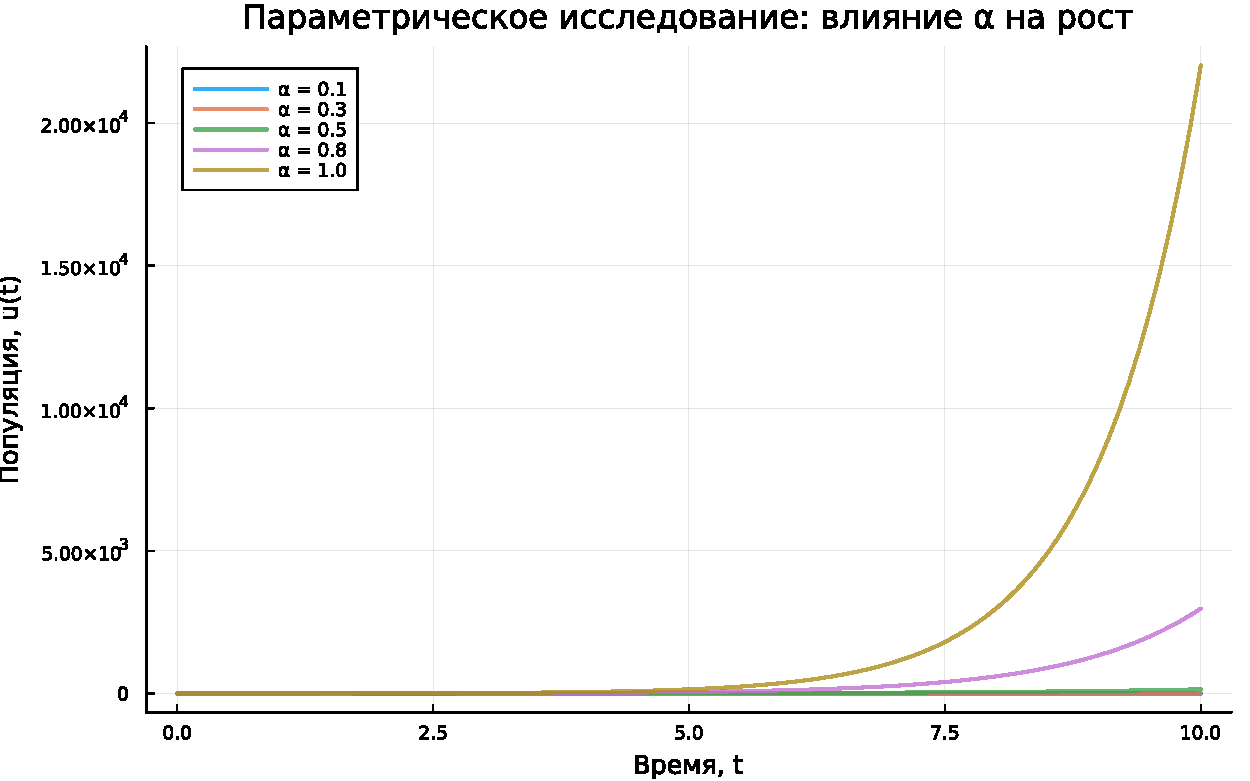
\includegraphics{mathmod-lab01-report-Nelia_files/mediabag/mathmod-lab01-report-Nelia_files/figure-pdf/cell-23-output-1.pdf}

Сохраним график в папку plots

\begin{Shaded}
\begin{Highlighting}[]
\FunctionTok{savefig}\NormalTok{(}\FunctionTok{plotsdir}\NormalTok{(script\_name, }\StringTok{"parametric\_scan\_comparison.png"}\NormalTok{))}
\end{Highlighting}
\end{Shaded}

\begin{verbatim}
"/home/nelianjovu/work/study/2026-1/2026-1==study--mathmod/2026-1--study--mathmod/labs/lab01/project/plots/parametric_scan_comparison.png"
\end{verbatim}

График зависимости времени удвоения от α

\begin{Shaded}
\begin{Highlighting}[]
\NormalTok{p3 }\OperatorTok{=} \FunctionTok{plot}\NormalTok{(results\_df.α, results\_df.doubling\_time,}
\NormalTok{    seriestype}\OperatorTok{=:}\NormalTok{scatter,}
\NormalTok{    label}\OperatorTok{=}\StringTok{"Численное решение"}\NormalTok{,}
\NormalTok{    xlabel}\OperatorTok{=}\StringTok{"Скорость роста, α"}\NormalTok{,}
\NormalTok{    ylabel}\OperatorTok{=}\StringTok{"Время удвоения, t₂"}\NormalTok{,}
\NormalTok{    title}\OperatorTok{=}\StringTok{"Зависимость времени удвоения от α"}\NormalTok{,}
\NormalTok{    markersize}\OperatorTok{=}\FloatTok{8}\NormalTok{,}
\NormalTok{    markercolor}\OperatorTok{=:}\NormalTok{red,}
\NormalTok{    legend}\OperatorTok{=:}\NormalTok{topright}
\NormalTok{)}
\end{Highlighting}
\end{Shaded}

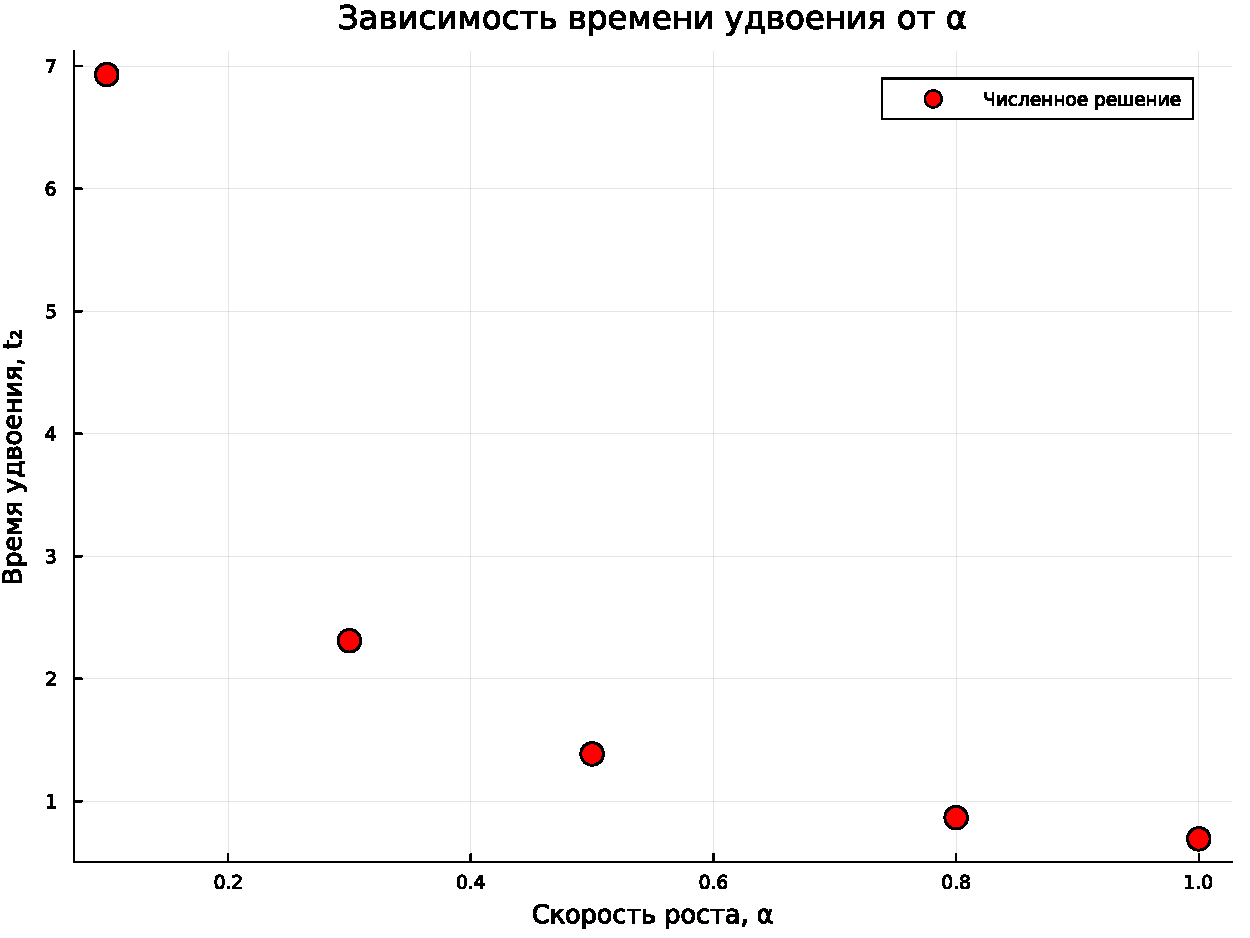
\includegraphics{mathmod-lab01-report-Nelia_files/mediabag/mathmod-lab01-report-Nelia_files/figure-pdf/cell-25-output-1.pdf}

Теоретическая кривая: t₂ = ln(2)/α

\begin{Shaded}
\begin{Highlighting}[]
\NormalTok{α\_range }\OperatorTok{=} \FloatTok{0.1}\OperatorTok{:}\FloatTok{0.01}\OperatorTok{:}\FloatTok{1.0}
\FunctionTok{plot!}\NormalTok{(p3, α\_range, }\FunctionTok{log}\NormalTok{(}\FloatTok{2}\NormalTok{) }\OperatorTok{./}\NormalTok{ α\_range,}
\NormalTok{    label}\OperatorTok{=}\StringTok{"Теория: t₂ = ln(2)/α"}\NormalTok{,}
\NormalTok{    lw}\OperatorTok{=}\FloatTok{2}\NormalTok{,}
\NormalTok{    linestyle}\OperatorTok{=:}\NormalTok{dash,}
\NormalTok{    linecolor}\OperatorTok{=:}\NormalTok{blue}
\NormalTok{)}
\end{Highlighting}
\end{Shaded}

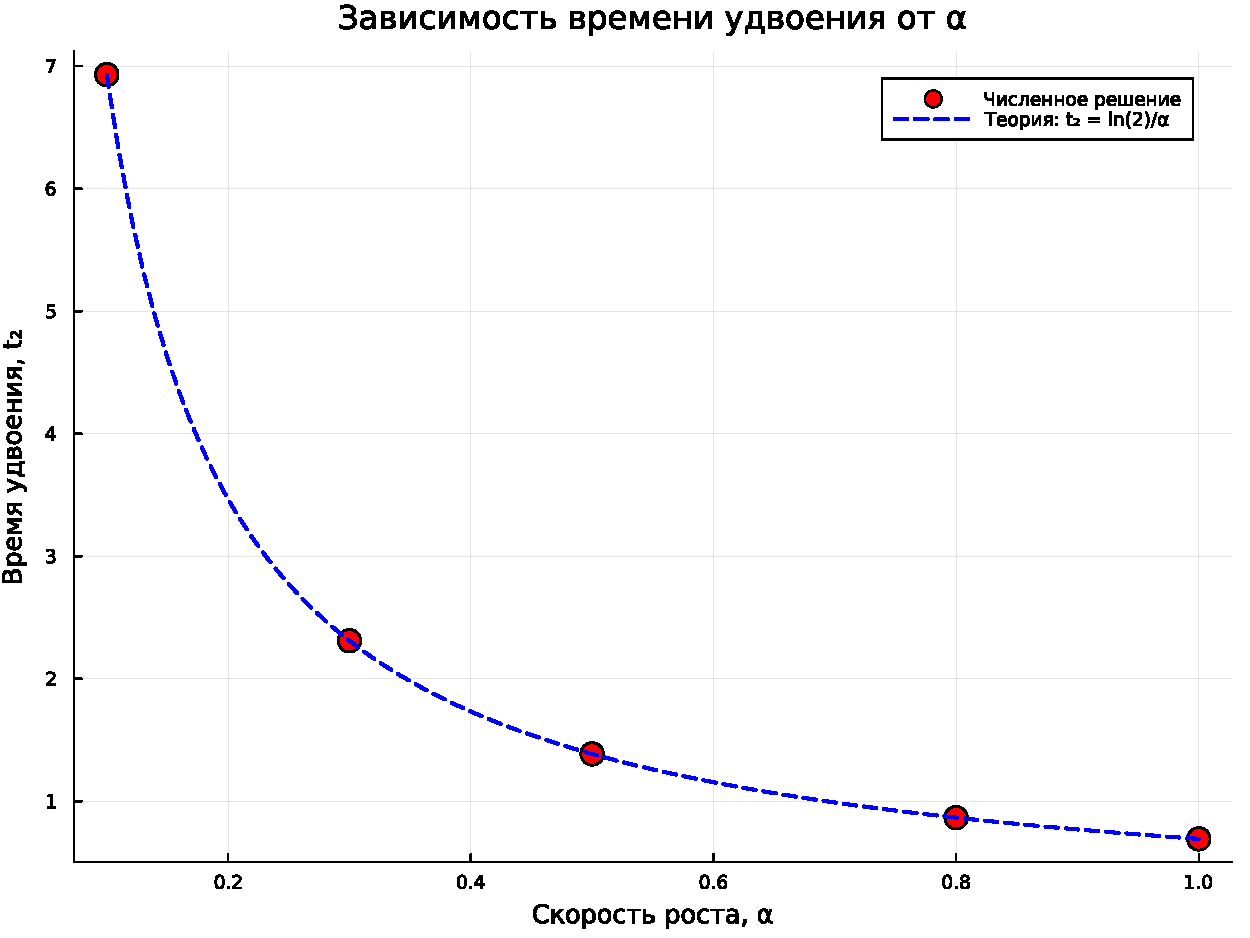
\includegraphics{mathmod-lab01-report-Nelia_files/mediabag/mathmod-lab01-report-Nelia_files/figure-pdf/cell-26-output-1.pdf}

Сохраним график в папку plots

\begin{Shaded}
\begin{Highlighting}[]
\FunctionTok{savefig}\NormalTok{(}\FunctionTok{plotsdir}\NormalTok{(script\_name, }\StringTok{"doubling\_time\_vs\_alpha.png"}\NormalTok{))}
\end{Highlighting}
\end{Shaded}

\begin{verbatim}
"/home/nelianjovu/work/study/2026-1/2026-1==study--mathmod/2026-1--study--mathmod/labs/lab01/project/plots/doubling_time_vs_alpha.png"
\end{verbatim}

\section{Бенчмаркинг с разными
параметрами}\label{ux431ux435ux43dux447ux43cux430ux440ux43aux438ux43dux433-ux441-ux440ux430ux437ux43dux44bux43cux438-ux43fux430ux440ux430ux43cux435ux442ux440ux430ux43cux438}

\textbf{ИЗМЕНЕНИЕ:} Бенчмаркинг для разных значений α

\begin{Shaded}
\begin{Highlighting}[]
\FunctionTok{println}\NormalTok{(}\StringTok{"}\SpecialCharTok{\textbackslash{}n}\StringTok{"} \OperatorTok{*} \StringTok{"="}\OperatorTok{\^{}}\FloatTok{60}\NormalTok{)}
\FunctionTok{println}\NormalTok{(}\StringTok{"Бенчмаркинг для разных значений α"}\NormalTok{)}
\FunctionTok{println}\NormalTok{(}\StringTok{"="}\OperatorTok{\^{}}\FloatTok{60}\NormalTok{)}

\NormalTok{benchmark\_results }\OperatorTok{=}\NormalTok{ []}

\ControlFlowTok{for}\NormalTok{ α\_value }\KeywordTok{in}\NormalTok{ param\_grid[}\OperatorTok{:}\NormalTok{α]}
\NormalTok{    bench\_params }\OperatorTok{=} \FunctionTok{Dict}\NormalTok{(}
        \OperatorTok{:}\NormalTok{u0 }\OperatorTok{=\textgreater{}}\NormalTok{ [}\FloatTok{1.0}\NormalTok{],}
        \OperatorTok{:}\NormalTok{α }\OperatorTok{=\textgreater{}}\NormalTok{ α\_value,}
        \OperatorTok{:}\NormalTok{tspan }\OperatorTok{=\textgreater{}}\NormalTok{ (}\FloatTok{0.0}\NormalTok{, }\FloatTok{10.0}\NormalTok{),}
        \OperatorTok{:}\NormalTok{solver }\OperatorTok{=\textgreater{}} \FunctionTok{Tsit5}\NormalTok{(),}
        \OperatorTok{:}\NormalTok{saveat }\OperatorTok{=\textgreater{}} \FloatTok{0.1}
\NormalTok{    )}

    \KeywordTok{function} \FunctionTok{benchmark\_run}\NormalTok{()}
\NormalTok{        prob }\OperatorTok{=} \FunctionTok{ODEProblem}\NormalTok{(exponential\_growth!,}
\NormalTok{            bench\_params[}\OperatorTok{:}\NormalTok{u0],}
\NormalTok{            bench\_params[}\OperatorTok{:}\NormalTok{tspan],}
\NormalTok{            (α}\OperatorTok{=}\NormalTok{bench\_params[}\OperatorTok{:}\NormalTok{α],))}
        \ControlFlowTok{return} \FunctionTok{solve}\NormalTok{(prob, bench\_params[}\OperatorTok{:}\NormalTok{solver]; saveat}\OperatorTok{=}\NormalTok{bench\_params[}\OperatorTok{:}\NormalTok{saveat])}
    \ControlFlowTok{end}

    \FunctionTok{println}\NormalTok{(}\StringTok{"}\SpecialCharTok{\textbackslash{}n}\StringTok{Бенчмарк для α = }\SpecialCharTok{$}\StringTok{α}\NormalTok{\_value}\StringTok{:"}\NormalTok{)}
\NormalTok{    b }\OperatorTok{=} \PreprocessorTok{@benchmark} \OperatorTok{$}\FunctionTok{benchmark\_run}\NormalTok{() samples}\OperatorTok{=}\FloatTok{100}\NormalTok{ evals}\OperatorTok{=}\FloatTok{1}
    \FunctionTok{push!}\NormalTok{(benchmark\_results, (α}\OperatorTok{=}\NormalTok{α\_value, time}\OperatorTok{=}\FunctionTok{median}\NormalTok{(b).time}\OperatorTok{/}\FloatTok{1e9}\NormalTok{))}
    \FunctionTok{println}\NormalTok{(}\StringTok{" Среднее время: "}\NormalTok{, }\FunctionTok{round}\NormalTok{(}\FunctionTok{median}\NormalTok{(b).time}\OperatorTok{/}\FloatTok{1e9}\NormalTok{, digits}\OperatorTok{=}\FloatTok{4}\NormalTok{), }\StringTok{" сек"}\NormalTok{)}
\KeywordTok{end}
\end{Highlighting}
\end{Shaded}

\begin{verbatim}

============================================================
Бенчмаркинг для разных значений α
============================================================

Бенчмарк для α = 0.1:
 Среднее время: 0.0001 сек

Бенчмарк для α = 0.3:
 Среднее время: 0.0001 сек

Бенчмарк для α = 0.5:
 Среднее время: 0.0001 сек

Бенчмарк для α = 0.8:
 Среднее время: 0.0001 сек

Бенчмарк для α = 1.0:
 Среднее время: 0.0001 сек
\end{verbatim}

График зависимости времени вычисления от α

\begin{Shaded}
\begin{Highlighting}[]
\NormalTok{bench\_df }\OperatorTok{=} \FunctionTok{DataFrame}\NormalTok{(benchmark\_results)}

\NormalTok{p4 }\OperatorTok{=} \FunctionTok{plot}\NormalTok{(bench\_df.α, bench\_df.time,}
\NormalTok{    seriestype}\OperatorTok{=:}\NormalTok{scatter,}
\NormalTok{    label}\OperatorTok{=}\StringTok{"Время вычисления"}\NormalTok{,}
\NormalTok{    xlabel}\OperatorTok{=}\StringTok{"Скорость роста, α"}\NormalTok{,}
\NormalTok{    ylabel}\OperatorTok{=}\StringTok{"Время вычисления, сек"}\NormalTok{,}
\NormalTok{    title}\OperatorTok{=}\StringTok{"Зависимость времени вычисления от α"}\NormalTok{,}
\NormalTok{    markersize}\OperatorTok{=}\FloatTok{8}\NormalTok{,}
\NormalTok{    markercolor}\OperatorTok{=:}\NormalTok{green,}
\NormalTok{    legend}\OperatorTok{=:}\NormalTok{topleft}
\NormalTok{)}
\end{Highlighting}
\end{Shaded}

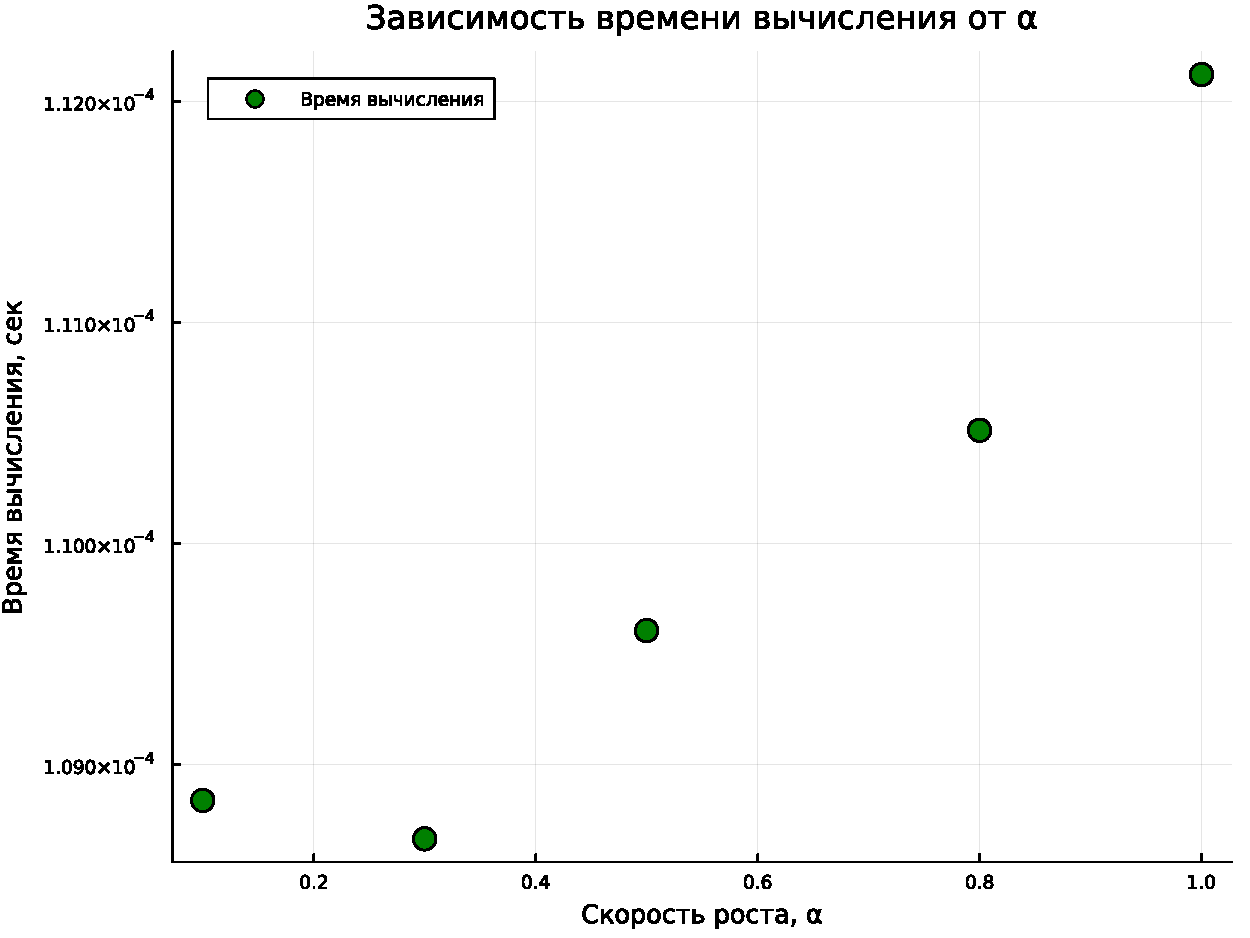
\includegraphics{mathmod-lab01-report-Nelia_files/mediabag/mathmod-lab01-report-Nelia_files/figure-pdf/cell-29-output-1.pdf}

Сохраним график в папку plots

\begin{Shaded}
\begin{Highlighting}[]
\FunctionTok{savefig}\NormalTok{(}\FunctionTok{plotsdir}\NormalTok{(script\_name, }\StringTok{"computation\_time\_vs\_alpha.png"}\NormalTok{))}
\end{Highlighting}
\end{Shaded}

\begin{verbatim}
"/home/nelianjovu/work/study/2026-1/2026-1==study--mathmod/2026-1--study--mathmod/labs/lab01/project/plots/computation_time_vs_alpha.png"
\end{verbatim}

\section{Сохранение всех
результатов}\label{ux441ux43eux445ux440ux430ux43dux435ux43dux438ux435-ux432ux441ux435ux445-ux440ux435ux437ux443ux43bux44cux442ux430ux442ux43eux432-1}

\textbf{НОВАЯ СЕКЦИЯ:} Сохранение сводных данных для последующего
анализа

\begin{Shaded}
\begin{Highlighting}[]
\PreprocessorTok{@save} \FunctionTok{datadir}\NormalTok{(script\_name, }\StringTok{"all\_results.jld2"}\NormalTok{) base\_params param\_grid all\_params results\_df bench\_df}
\PreprocessorTok{@save} \FunctionTok{datadir}\NormalTok{(script\_name, }\StringTok{"all\_plots.jld2"}\NormalTok{) p1 p2 p3 p4}

\FunctionTok{println}\NormalTok{(}\StringTok{"}\SpecialCharTok{\textbackslash{}n}\StringTok{"} \OperatorTok{*} \StringTok{"="}\OperatorTok{\^{}}\FloatTok{60}\NormalTok{)}
\FunctionTok{println}\NormalTok{(}\StringTok{"ЛАБОРАТОРНАЯ РАБОТА ЗАВЕРШЕНА"}\NormalTok{)}
\FunctionTok{println}\NormalTok{(}\StringTok{"="}\OperatorTok{\^{}}\FloatTok{60}\NormalTok{)}

\FunctionTok{println}\NormalTok{(}\StringTok{"}\SpecialCharTok{\textbackslash{}n}\StringTok{Результаты сохранены в:"}\NormalTok{)}
\FunctionTok{println}\NormalTok{(}\StringTok{" • data/}\SpecialCharTok{$}\NormalTok{(script\_name)}\StringTok{/single/ {-} базовый эксперимент"}\NormalTok{)}
\FunctionTok{println}\NormalTok{(}\StringTok{" • data/}\SpecialCharTok{$}\NormalTok{(script\_name)}\StringTok{/parametric\_scan/ {-} параметрическое сканирование"}\NormalTok{)}
\FunctionTok{println}\NormalTok{(}\StringTok{" • data/}\SpecialCharTok{$}\NormalTok{(script\_name)}\StringTok{/all\_results.jld2 {-} сводные данные"}\NormalTok{)}
\FunctionTok{println}\NormalTok{(}\StringTok{" • plots/}\SpecialCharTok{$}\NormalTok{(script\_name)}\StringTok{/ {-} все графики"}\NormalTok{)}
\FunctionTok{println}\NormalTok{(}\StringTok{" • data/}\SpecialCharTok{$}\NormalTok{(script\_name)}\StringTok{/all\_plots.jld2 {-} объекты графиков"}\NormalTok{)}

\FunctionTok{println}\NormalTok{(}\StringTok{"}\SpecialCharTok{\textbackslash{}n}\StringTok{Для анализа результатов используйте:"}\NormalTok{)}
\FunctionTok{println}\NormalTok{(}\StringTok{" using JLD2, DataFrames"}\NormalTok{)}
\FunctionTok{println}\NormalTok{(}\StringTok{" @load }\SpecialCharTok{\textbackslash{}"}\StringTok{data/}\SpecialCharTok{$}\NormalTok{(script\_name)}\StringTok{/all\_results.jld2}\SpecialCharTok{\textbackslash{}"}\StringTok{"}\NormalTok{)}
\FunctionTok{println}\NormalTok{(}\StringTok{" println(results\_df)"}\NormalTok{)}
\end{Highlighting}
\end{Shaded}

\begin{verbatim}

============================================================
ЛАБОРАТОРНАЯ РАБОТА ЗАВЕРШЕНА
============================================================

Результаты сохранены в:
 • data//single/ - базовый эксперимент
 • data//parametric_scan/ - параметрическое сканирование
 • data//all_results.jld2 - сводные данные
 • plots// - все графики
 • data//all_plots.jld2 - объекты графиков

Для анализа результатов используйте:
 using JLD2, DataFrames
 @load "data//all_results.jld2"
 println(results_df)
\end{verbatim}

\chapter{Выводы}\label{ux432ux44bux432ux43eux434ux44b}

Делая эту лабораторную работу, я изучила модель экспоненциального роста
и проверила параметрическое исследование влияния коэффициента роста α на
динамику системы, а также освоила современные практики воспроизводимых
исследований (литературное программирование, DrWatson, Git).

\chapter*{Список
литературы}\label{ux441ux43fux438ux441ux43eux43a-ux43bux438ux442ux435ux440ux430ux442ux443ux440ux44b}
\addcontentsline{toc}{chapter}{Список литературы}

\begin{enumerate}
\def\labelenumi{\arabic{enumi}.}
\item
  A Multi-Language Computing Environment for Literate Programming and
  Reproducible Research / E. Schulte {[}et al.{]} // Journal of
  Statistical Software. --- 2012. --- Vol. 46, no. 3. --- ISSN
  1548-7660. --- DOI: 10.18637/jss.v046.i03.
\item
  Knuth D. E. Literate Programming // The Computer Journal. --- 1984.
  --- Feb.~--- Vol. 27, no. 2. --- P. 97--111. --- ISSN 1460-2067. ---
  DOI: 10.1093/comjnl/27.2.97.
\item
  The Story in the Notebook / M. B. Kery {[}et al.{]} // Proceedings of
  the 2018 CHI Conference on Human Factors in Computing Systems. ---
  ACM, 04/2018. --- P. 1--11. --- DOI: 10.1145/3173574.3173748.
\end{enumerate}


\printbibliography


\end{document}
